% !TEX encoding = ISO-8859-1
\documentclass[bsc,oneside]{ufpethesis}

% \usepackage[T1]{fontenc}

\usepackage{amssymb}
\usepackage{amsmath}
\usepackage{mathtools}
\usepackage{hyperref}
\usepackage{algorithm}
\usepackage{algorithmic}
\usepackage{subfigure}
\usepackage{appendix}

\algsetup{linenosize=\small,linenodelimiter=.}
\hypersetup{colorlinks,citecolor=black,filecolor=black,linkcolor=black,urlcolor=black}

\usepackage{amsthm}

% \university{<NOME DA UNIVERSIDADE>} default: UFPE
% \address{<CIDADE DA IES>} default: UFPE
\institute{Centro de Inform�tica}
% \department{<NOME DO DEPARTAMENTO>} n�o se aplica
\program{Gradua��o em Engenharia da Computa��o}
\majorfield{Engenharia da Computa��o}
\title{An�lise comparativa de t�cnicas de sele��o de prot�tipos}
\date{22 de novembro de 2011}

\author{Dayvid Victor Rodrigues de Oliveira}
\adviser{Prof. Dr. George Darmiton}
% \coadviser{NOME DO(DA) CO-ORIENTADOR(A)} n�o se aplica

%% Inicio do documento
\begin{document}

\frontmatter
% Folha de rosto
\frontpage
% Portada (apresenta��o)
\presentationpage

% Dedicat�ria
\begin{dedicatory}
Eu dedico este trabalho a Jo�o Rodrigues de Silva, meu av�.
\end{dedicatory}

% Agradecimentos
\acknowledgements
Agrade�o a Deus.
% % !TEX encoding = ISO-8859-1

Senhor, obrigado por ter me dado a força e a confiança para completar esta jornada,\\
obrigado por ter me guiado através de todos os obstáculos no meu caminho,\\
e por me manter \\
obrigado pela tua proteção em todo caminho,\\
obrigado pelos amigos que eu fiz,\\
que o Senhor cuide deles, assim como cuidou de mim,\\
obrigado por me permitir (...)


\begin{epigraph}[Boston, 2001]{Bono}
What can I give back to God, for the blessings You pour out on me?
\end{epigraph}

% Resumo em Portugu�s
% Se preferir, crie um arquivo � parte e o inclua via \include{}
\resumo
RESUMO
% Palavras-chave do resumo em Portugu�s
\begin{keywords}
PORTUGUES
\end{keywords}

% Resumo em Ingl�s
% Se preferir, crie um arquivo � parte e o inclua via \include{}
\abstract
ABSTRACT
\begin{keywords}
INGLES
\end{keywords}

\tableofcontents
\listoffigures
\listoftables

\mainmatter

% !TEX encoding = ISO-8859-1
\chapter{Introdu��o}
% \label{ch:introducao}

Neste cap�tulo ser� dada uma introdu��o � sele��o de prot�tipos. Para melhor entendimento deste assunto, ser�o apresentados contexto hist�rico, motiva��o do uso de sele��o de prot�tipos, e os desafios atuais.

Logo depois da sess�o de motiva��o e contextualiza��o, seguir� um detalhamento deste trabalho, abordando objetivo e estrutura do mesmo.

\section{Motiva��o e Contextualiza��o}

\subsection{Hist�rico}

No final dos anos 50, surgiram os primeiros trabalhos de aprendizagem de m�quina. De uma forma geral, elas consistiam em dar ao computador a habilidade de reconhecer formas. A partir da�, surgiram diversos problemas onde a aprendizagem de m�quina atuava. 

Existem tr�s problemas gerais que a aprendizagem de m�quina tenta resolver. Um deles � o problema do agrupamento, que consiste em agrupar dados de acordo com suas caracter�sticas, de forma que seja poss�vel extrair informa��o �til desdes agrupamentos. Um outro problema � a discrimina��o, que basicamente � achar uma forma de reconhecer um conceito, dado um conjunto de conceitos exemplos. O terceiro e �ltimo problema, � o da generaliza��o, que � o problema de como reduzir uma regra, tornando-a mais abrangente e menos custosa.

Reconhecimento de padr�es ataca principalmente o problema da discrimina��o, tendo por objetivo classificar padr�es, discriminando-os entre duas ou mais classes. A classifica��o pode ser feita com padr�es pertencentes a qualquer dom�nio, como reconhecimento de digitais, gestos, escrita, fala, entre outros.

Todo sistema de reconhecimento de padr�es utiliza um classificador para discriminar os padr�es de teste. O quanto um dado classificador � eficiente � medido pela taxa de acerto m�dia, pela vari�ncia, e pela efici�ncia em termos de custo computacional. Um classificador de aprendizagem baseada em inst�ncias muito utilizado � o \textit{K-Nearest Neighbor}, KNN \cite{knnrule:1969}. 

O KNN � muito usado por ser um m�todo de aprendizagem supervisionado simples, e por possuir uma taxa de acerto relativamente alta. O conceito b�sico consiste em: Dado um padr�o $x$ a ser classificado e um conjunto de padr�es conhecidos $T$, obter as classes dos $K$ elementos de $T$ mais pr�ximos de $x$. A classe que obtiver maior ocorr�ncia, ou peso, ser� a classe de $x$. Pode-se dizer que o KNN utiliza uma abordagem \textit{"Dize-me com quem andas, e direi quem �s."}. O algoritmo esta descrito em Algorithm \ref{alg:knn}.

\begin{algorithm}[H]
\caption{KNN}
\label{alg:knn}
\begin{algorithmic}[1]
\REQUIRE {$K$: um n�mero}
\REQUIRE {$T$: conjunto de treinamento}
\REQUIRE {$x$: elemento para ser classificado}
\REQUIRE {$L$: uma lista}
\FORALL {$t_i$ $\in$ $T$}
\STATE  $d_i$ = $distance(t_i, x)$
\STATE  adicione $(d_i, Classe(t_i))$ em $L$
\ENDFOR
\STATE $Ordene(L)$ de acordo com as dist�ncias
\STATE obtenha os $K$ primeiros elementos de $L$
\RETURN a classe de maior ocorr�ncia, ou peso, entre os $K$
\end{algorithmic}
\end{algorithm}


Conforme mostrado em Algorithm \ref{alg:knn}, o KNN � muito simples, por�m, possui um custo alto, pois precisa visitar todos os elementos da base de dados para realizar uma classifica��o. Assim sendo, � preciso resolver o problema de agrupamento e generaliza��o. Uma das abordagens utilizadas � a sele��o de prot�tipos, detalhada na pr�xima subsess�o.


\subsection{Sele��o de Prot�tipos}

A estrat�gia do KNN, apesar de eficiente, possui algumas desvantagens. A primeira desvantagem � que o KNN � sens�vel � ru�dos, para baixos valores de K. Outra desvantagem � que o KNN � custoso, pois precisa calcular a dist�ncia do padr�o que se deseja classificar para cada um dos padr�es da base de treinamento, com isso, o KNN torna-se lento em rela��o a outros classificadores.

Para resolver este problema, surgiu a id�ia de utilizar um conjunto menor, gerado a partir da base de dados original (conjunto de treinamento), que represente bem todas as classes, este processo � chamado de sele��o de prot�tipos. A escolha dos prot�tipos deve ser feita cuidadosamente, pois � necess�rio que estes elementos possuam uma boa representatividade de todo o conjunto de treinamento. � importante tamb�m, que os prot�tipos n�o sejam elementos ruidosos, pois isso compromete a taxa de acerto do classificador.

Com os prot�tipos gerados � poss�vel utilizar o \textit{Nearest Prototype Classification}, NPC, que � utilizar prot�tipos gerados como treinamento do KNN. Assim a base de dados � reduzida, diminuindo o espa�o de armazenamento e o tempo de processamento. Na figura \ref{fig:npc} percebe-se a redu��o obtida com o uso de sele��o de prot�tipos.

\begin{figure}[H]
\center
\label{fig:npc}
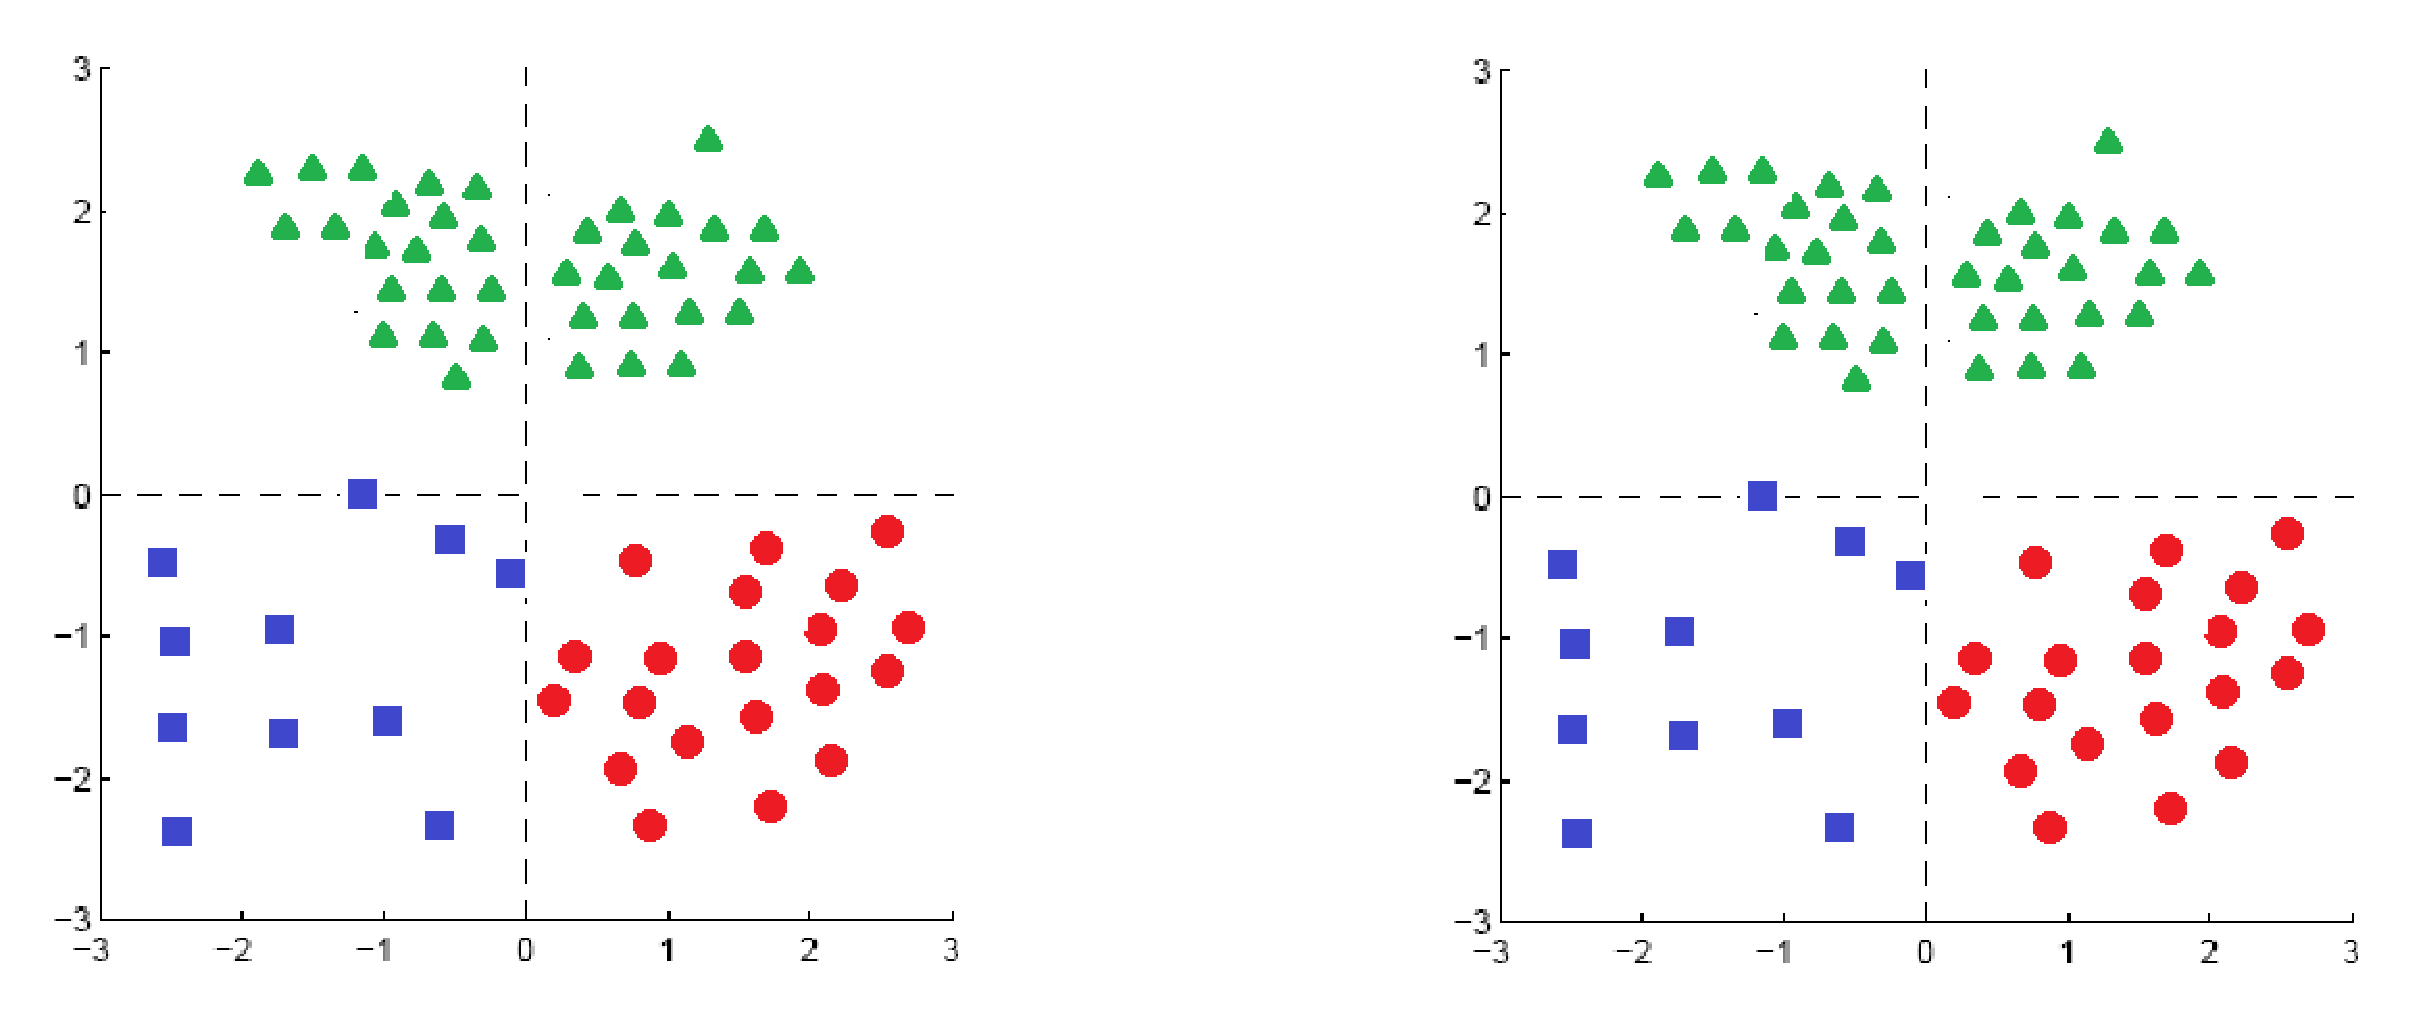
\includegraphics[scale=0.40]{imagens/npc.eps}
\caption{Exemplo do NPC}
\end{figure}

Al�m de possuir vantagens gerais como a diminui��o do espa�o de armazenamento e redu��o de esfor�o computacional para classifica��o, a sele��o de prot�tipos pode ainda aumentar o desempenho do classificador. Esta melhora acontece com a elimina��o de ru�dos e outliers, pois os prot�tipos aumentam a capacidade de generaliza��o do classificador, levando a maiores taxas de acerto.

Algumas t�cnicas de sele��o de prot�tipos selecionam inst�ncias que pertecem ao conjunto de treinamento, ou seja, elas escolhem, dentre as inst�ncias utilizadas, aquelas que julgam ser mais apropriadas para serem prot�tipos. T�cnicas que utilizam esta abordagem s�o chamadas de puramente seletivas. Exemplos de t�cnicas seletivas s�o \textit{Edited Nearest Neighbor} \cite{enn:2011}, \textit{Condensed Nearest Neighbor} \cite{cnn:1968}, \textit{Tomek Links} e \textit{One-Sided Selection} \cite{conf/icml/KubatM97}.

Outras t�cnicas criam novos elementos durante o processo de redu��o, os prot�tipos s�o criados atrav�s de combina��o entre as inst�ncias do conjunto de original e ajustes relizados por meio de treinamento supervisionado. Estas t�cnicas s�o chamadas de criativas, entre elas est�o \textit{Learning Vector Quantization 1, 2.1 e 3} \cite{kohonen:lvq} e \textit{Self-Generating Prototypes}\cite{fayed:sgp}.

T�cnicas de sele��o de prot�tipos tamb�m podem ser classificadas como determin�sticas ou n�o deterministicas. T�cnicas determin�sticas s�o aquelas que, dada uma base de dados, sempre ser� gera o mesmo conjunto de prot�tipos, independente da ordem em que as inst�ncias de treinamento s�o apresentadas. T�cnicas n�o determin�sticas s�o aquelas que dependem da ordem das inst�ncias de treinamento, ou dependem de inst�ncias pr�-selecionadas para ajuste posterior.

Cada uma das t�cnicas de sele��o de prot�tipos aprensentam caracter�sticas pr�prias, sendo necess�rio uma an�lise do quanto cada uma destas t�cnicas � apropriada para um dado tipo de base de dados. Algumas t�cnicas removem inst�ncias redundantes, outras, removem inst�ncias que est�o na fronteira de classifica��o, e outras fazem uma combina��o das duas abordagens. Detalhes de algumas destas t�cnicas ser�o mostrados no pr�ximo cap�tulo.

\subsection{Bases Desbalanceadas}

Em v�rias situa��es do mundo real, os classificadores precisam ser treinados com bases de dados que possue muito mais inst�ncias de uma de uma classe do que das outras classes, tais bases de dados s�o chamadas de bases desbalanceadas. Quanto maior a diferen�a entre a quantidade de inst�ncias de cada classe, maior o n�vel de desbalanceamento da base.

Quando treinados com bases de dados desbalanceadas, classificadores sofrem uma redu��o da performace, e normalmente tendem a classificar mais padr�es com as classes marjorit�rias. Este � um problema grave, visto que, normalmente, a classifica��o de inst�ncias da classe minorit�ria � que s�o mais importantes (como exemplo, informa��es sobre doen�as) \cite{conf/icml/HulseKN07}.

Da mesma forma que classificadores podem ser prejudicados por um desbalanceamento, t�cnicas de sele��o de prot�tipos podem sofrer da mesma forma, selecionando muitas inst�ncias da classe marjorit�ria e poucas, ou nenhuma, da classe minorit�ria.

\section{Objetivo}

O objetivo deste trabalho � expor algumas t�cnicas de sele��o de prot�tipos e avaliar seu desempenho em bases desbalanceadas. A avalia��o de desempenho se refere a taxa de acerto utilizando bases de dados reais, e a disposi��o dos prot�tipos por meio de bases artificiais de diferentes n�veis de desbalanceamento e sobreposi��o de classes.

Para que o trabalho seja mais objetivo, apenas os exemplos mais interessante de cada t�cnica de sele��o de prot�tipos ser�o enfatizados, citando as maiores vantagens e desvantagens de cada uma delas.

No final do trabalho, ser� poss�vel identificar quais t�cnicas s�o mais apropriadas para bases de dados desbalanceadas, e possivelmente propor adapta��es para otimizar algumas delas.

\section{Estrutura do Trabalho}

O restante deste trabalho possui um cap�tulo com detalhes sobre diferentes t�cnicas de sele��o de prot�tipos. Durante o cap�tulo, ser�o citadas as caracter�sticas e adapta��es j� conhecidas para tratar de bases desbalanceadas, assim como ilustra��es e algoritmos.

Logo ap�s, segue um cap�tulo mostrando casos de sucesso e falha de cada t�cnica em bases de dados artificiais, e por fim, um cap�tulo mostrado os resultados em bases de dados reais com conclus�es.

As an�lises levar�o em conta a disposi��o e a quantidade dos prot�tipos resultantes de cada t�cnica. Al�m disso, ser� calculada a taxa de acerto dos prot�tipos em rela��o ao pr�prio conjunto de treinamento para analisar a representatividade. Por fim, cada t�cnica ser� executada em bases de dados reais, onde ser� utilizada \textit{K-Fold Cross-Validation} para calcular a taxa de acerto m�dia de cada t�cnica.

% !TEX encoding = ISO-8859-1
\chapter{T�cnicas de Sele��o de Prot�tipos}
% \label{ch:tecnicasdeselecaodeprototipos}

Neste cap�tulo, ser�o mostradas as t�cnicas de sele��o de prot�tipos abordadas neste trabalho. Cada uma das sess�es abaixo abordar� uma t�cnica, ser� mostrado o conceito da t�cnica, assim como o pseudo-c�digo e as caracter�sicas de cada uma destas t�cnicas.

\section{ENN}

Edited Nearest Neighbor Rule\cite{enn:2011} � uma t�cnica de sele��o de prot�tipos puramente seletiva proposta por Wilson em 1976. De uma forma geral, esta t�cnica foi projetada para funcionar como um filtro de ru�dos, ela elimina pontos na regi�o de fronteira, regi�o de alta susceptibilidade a erros, e com isso elimina ru�dos.\

Por atuar apenas na regi�o de fronteira, esta t�cnica possui uma baixa capacidade de redu��o, deixando as inst�ncias que n�o se encontram na regi�o de fronteira intactas, exceto pelos ru�dos extremos.\

Uma desvantagem desta t�cnica � que ela possui uma baixa capacidade de redu��o de elementos, visto que ela n�o elimina redund�ncia.

Segue abaixo o algoritmo da execu��o do ENN e, logo ap�s, alguns coment�rios sobre este algoritmo.

\begin{algorithm}
\caption{ENN}
\label{pseudocode_enn}
\begin{algorithmic}[1]
\REQUIRE {$list$: uma lista}
\FORALL {inst�ncia $e_i$ da base de dados original}
\STATE Aplique o KNN sobre $e_i$
\IF {$e_i$ foi classificado erroneamente}
\STATE salve $e_i$ em $list$
\ENDIF
\ENDFOR
\STATE Remova da base de dados todos os elementos que est�o em $list$
\end{algorithmic}
\end{algorithm}

O valor de K pode variar de acordo com o tamanho da base de dados, por�m, tipicamente, utiliza-se o valor de K=3. Tipicamente, O valor de K � inversamente proporcional a quantidade de inst�ncias que ser�o eliminadas, ou seja, para que o filtro elimine todos os poss�veis ru�dos, deve-se utilizar K=1.

%% TODO COLOCAR ALGUMA FIGURA PARA EXEMPLIFICAR
%% TODO EXPLICAR A FIGURA

Uma vantagem do ENN � que ele independe da ordem que a base de dados foi apresentada, ou seja, o ENN aplicado a uma base de dados, com o mesmo valor de K, sempre ter� o mesmo resultado.

%% TODO CITAR DESVANTAGENS DO ENN 

\section{CNN}

Condensed Nearest Neighbor \cite{cnn:1968} � uma t�cnica de sele��o de prot�tipos puramente seletiva que tem como objetivo eliminar informa��o redundante. Diferentemente do ENN \cite{enn:2011}, o CNN n�o elimina inst�ncias nas regi�es de fronteira, a t�cnica mant�m estes elementos pois estes que "s�o importantes" para distinguir entre duas classes.

A ideia geral do CNN � encontrar o menor subconjunto da base de dados original que, utilizando o 1-NN, classifica todos os padr�es da base de dados original corretamente. Fazendo isso, o algoritmo elimina os elementos mais afastados da regi�o de indecis�o, da fronteira de classifica��o.

O algoritmo do CNN ser� mostrado abaixo, e logo ap�s, coment�rios a respeito do mesmo.

\begin{algorithm}
\caption{CNN}
\label{pseudocode_cnn}
\begin{algorithmic}[1]
\REQUIRE {$list$: uma lista}
\STATE Escolha um elemento de cada classe $aleatoreamente$ e coloque-os em $list$
\FORALL {inst�ncia $e_i$ da base de dados original}
\STATE Aplique o KNN sobre $e_i$ utilizando os elementos em $list$ para treinamento
\IF {$e_i$ foi classificado erroneamente}
\STATE salve $e_i$ em $list$
\ENDIF
\ENDFOR
\STATE Remova da base original todos os elementos que n�o est�o em $list$
\end{algorithmic}
\end{algorithm}

Podemos observar que este algoritmo possui uma abordagem diferente do ENN, por exemplo, pois ele come�a com um conjunto m�nimo de inst�ncias (uma de cada classe) e depois adiciona inst�ncias conforme a necessidade de mant�-las para que todos os elementos da base de dados original sejam classificados corretamente.

Uma coisa que pode-se observar no algoritmo, � a palavra $aleatoriamente$, o que significa que o CNN aplicado numa mesma base de dados com um mesmo valor de K para o KNN, nem sempre resulta nos mesmos prot�tipos. O primeiro fato para que isso ocorra � a sele��o aleat�ria dos prot�tipos iniciais. Existem algumas adapta��es para o CNN, onde os prot�tipos iniciais s�o escolhidos utilizando t�cnicas como o SGP\cite{fayed:sgp} para obter as inst�ncias mais centrais. Modifica��es no CNN s�o muito comuns \cite{cnn:1976}, por�m, mesmo com estas modifica��es, o CNN ainda n�o � determin�stico, pois a ordem em que as inst�ncias s�o classificadas afeta o resultado final.

%% TODO COLOCAR ALGUMA FIGURA PARA EXEMPLIFICAR
%% TODO EXPLICAR A FIGURA

Para o caso de estudo abordado neste trabalho, o CNN pode ser utilizado de forma adaptada. A adapta��o consiste em manter todos os elementos da classe minorit�ria e o m�nimo poss�vel da classe marjorit�ria. O pr�prio CNN se encarrega de remover os elementos redundantes da classe marjorit�ria, assim, basta apenas selecionar todos os elementos da classe minorit�ria aos prot�tipos iniciais.
Segue abaixo o algoritmo desta adapta��o:

\begin{algorithm}
\caption{CNN para bases desbalanceadas}
\label{pseudocode_cnn}
\begin{algorithmic}[1]
\REQUIRE {$list$: uma lista}
\STATE Coloque todos os elementos da classe minorit�ria em $list$
\FORALL {inst�ncia $e_i$ da base de dados original}
\STATE Aplique o KNN sobre $e_i$ utilizando os elementos em $list$ para treinamento
\IF {$e_i$ foi classificado erroneamente}
\STATE salve $e_i$ em $list$
\ENDIF
\ENDFOR
\STATE Remova da base original todos os elementos que n�o est�o em $list$
\end{algorithmic}
\end{algorithm}

Com o algoritmo CNN adaptado para bases desbalanceadas, os elementos redundantes da classe marjorit�ria s�o removidos, e todos os elementos da classe minorit�ria s�o mantidos. Esta adapta��o do CNN ir� reduzir a base de dados, ocasionando as vantagens de redu��o, e ainda reduzir� o desbalenceamento da base.


\section{Tomek Links}

Mantendo a mesma linha do ENN, Tomek Links � uma t�cnica de sele��o de prot�tipos puramente seletiva que elimina os elementos das regi�es de fronteiras e inst�ncias com probabilidade de ser ru�do. Tomek Links podem ser definidos da seguinte forma: Dadas duas inst�ncias $e_i$ e $e_j$, o par \textit{($e_i$, $e_j$)} � chamado de Tomek Link se n�o existe nenhuma inst�ncia $e_k$, tal que, para todo $e_k$ \textit{dist($e_i$,$e_j$) < dist($e_i$,$e_k$)} e \textit{dist($e_i$,$e_j$) < dist($e_j$,$e_k$)}. Segue abaixo o algor�tmo detalhado:

\begin{algorithm}
\caption{Seleciona Tomek Links}
\label{pseudocode_cnn}
\begin{algorithmic}[1]
\REQUIRE {$list$: uma lista}
	\FORALL {inst�ncia $e_i$ da base de dados original}
		\STATE $e_j$ = inst�ncia mais pr�xima de $e_i$
		\IF {inst�ncia mais p�oxima de $e_j$ for $e_i$}
			\IF {classe de $e_i$ for diferente da classe de $e_j$}
				\STATE salve o par \textit{($e_i$, $e_j$)} em $list$
			\ENDIF
		\ENDIF
	\ENDFOR
	\STATE Retorne os pares em $list$, os Tomek Links
\end{algorithmic}
\end{algorithm}



Os Tomek Links representam elementos da regi�o de fronteira e prov�veis ru�dos, e a t�cnica de sele��o de prot�tipos consiste em remover os Tomek Links da base de dados original. Segue abaixo o algoritmo da sele��o de prot�tipos:



\begin{algorithm}
\caption{Tomek Links}
\label{pseudocode_cnn}
\begin{algorithmic}[1]
\REQUIRE {$list$: uma lista}
\STATE $list$ = $Seleciona Tomek Links$ da base original
	\FORALL {\textit{($e_i$, $e_j$)} em $list$}
		\STATE remova $e_i$ da base original
		\STATE remova $e_j$ da base original
	\ENDFOR
	\STATE Retorne a base original filtrada
\end{algorithmic}
\end{algorithm}



Enquanto o CNN remove os elementos que est�o longe da regi�o de indecis�o, o Tomek Links remove os elementos que est�o pr�ximos desta regi�o, o que causa uma maior separa��o entre as classes.



%% TODO FIGURA PARA TOMEK LINKS
%% EXPLICAR FIGURA



Observa-se facilmente que os Tomek Links pode remove todas as inst�ncias da fronteira, inclusive as inst�ncias da classe minorit�ria, assim sendo, uma poss�vel adapta��o dos Tomek Links � eliminar apenas os elementos das classes marjorit�rias. Nesse caso, ainda ocorreria uma separa��o entre as classes, mas apenas as inst�ncias da classe marjorit�ria seriam removidos, dimunuindo assim o n�vel de desbalanceamento. Segue abaixo o algoritmo desta adapta��o:



\begin{algorithm}
\caption{Tomek Links}
\label{pseudocode_cnn}
\begin{algorithmic}[1]
\REQUIRE {$list$: uma lista}
	\STATE $list$ = $Seleciona Tomek Links$ da base original
	\FORALL {\textit{($e_i$, $e_j$)} em $list$}
		\IF {$e_i$ for da classe marjorit�ria}
			\STATE remova $e_i$ da base original
		\ENDIF
		\IF {$e_j$ for da classe marjorit�ria}
			\STATE remova $e_j$ da base original
		\ENDIF
	\ENDFOR
	\STATE Retorne a base original filtrada
\end{algorithmic}
\end{algorithm}



Com esta adapta��o, a classe minorit�ria � mantida, evitando o aumento do desbalanceamento ou a remo��o por alta probabilidade de ru�do.



\section{LVQ}
\subsection{LVQ 1}
\subsection{LVQ 2.1}
\subsection{LVQ 3}
\section{SGP}
\section{SGP 2}
\section{CCNN}



% !TEX encoding = ISO-8859-1
\chapter{An�lise em Bases Artificiais}
\label{ch:analiseembasesartificiais}

Neste cap�tulo ser� analisado o desempenho de cada t�cnica de sele��o de prot�tipos em bases desbalanceadas artificiais. Al�m da taxa de acerto, ser� considerada a quantidade de prot�tipos gerados por cada t�cnica e a distribui��o destes prot�tipos.

\section{Bases Artificiais}
\label{sec:basesartificiais}

Para avaliar de forma visual o comportamento de cada algoritmo de sele��o de prot�tipos, foram selecionadas bases artificiais com diferentes n�veis de sobrebosi��o entre a classe marjorit�ria e a classe minotir�ria. Tamb�m foram selecionados dois diferentes n�veis de desbalanceamento, um com aproximadamente 10\% de desbalanceamento e outro com aproximadamente 5\%.

No ap�ndice \ref{ch:appendixa}, p�gina \pageref{ch:appendixa}, est�o as figuras das bases de dados geradas artificialmente que ser�o utilizadas neste trabalho. Na figura \ref{fig:orig10} est�o os diferentes n�veis de sobreposi��o para uma base onde a classe minorit�ria possui 10\% das inst�ncias. O mesmo acontece na figura \ref{fig:orig5}, onde a classe minorit�ria possui apenas 5\% das inst�ncias.

Foi utilizado dois n�veis de desbalanceamento diferentes para avaliar se as t�cnicas tem o mesmo comportamento quando o n�vel de desbalanceamento � alterado.


\section{An�lise Individual}

Nesta sess�o, cada t�cnica sera analisada isoladamente. Para exemplificar e demonstrar as falhas de cada t�cnica, ser�o utilizadas figuras e tabelas que comprovem o comportamento de cada algoritmo diante de bases desbalanceadas.

Todas as conclus�es poder�o ser validadas ou mesmo reavaliadas com a aplica��o das t�cnicas de sele��o de prot�tipos em bases reais no pr�ximo cap�tulo.


\subsection{ENN}
\label{subsec:ennembasesartificiais}

	Conforme dito no cap�tulo anterior, o ENN � uma t�cnica que elimina ru�dos na fronteira de classifica��o, mantendo inst�ncias que apresentam redund�ncia de informa��o. Na tabela \ref{tab:enn5}, podemos ver a taxa de acerto do ENN em uma base com 10\%, onde o n�vel de sobreposi��o varia gradualmente, sendo o �ltimo n�vel o caso onda a classe minorit�ria est� totalmente imersa dentro da classe marjorit�ria, lembrando que, foi utilizado o pr�prio treinamento para teste, afim de avaliar a representatividade dos dados em rela��o a base original.

	Observa-se que a o ENN manteve uma boa taxa de acerto geral, sendo o pior caso com 94.74\%. Por�m, vemos que esta taxa diminui conforme o n�vel de sobreposi��o aumenta, na mesma propor��o em que inst�ncias s�o eliminadas. Por�m, ao observar a taxa de acerto da classe minorit�ria, pode-se perceber que o ENN eliminou muito mais inst�ncias da classe minorit�ria que da marjorit�ria.
	Inicialmente o n�vel de sobreposi��o das classes � zero, ent�o nenhuma inst�ncia � eliminada e a taxa de acerto � mantida. Conforme o n�vel de sobreposi��o das classes vai aumentnado, a taxa de acerto da classe minorit�ria vai decrescendo, chegando at� 0\% quando a classe minorit�ria est� totalmente sobreposta. Na tabela \ref{tab:enn10} acontece o mesmo, por�m, o decrescimento da taxa de acerto da classe minorit�ria � menor.


\begin{table}[H]
\begin{center}
\begin{tabular}{|l|l|l|l|l|l|}
\hline
N�vel de Intersec��o    &   I   &   II  &   III &   IV  &   V   \\
\hline %----- linha horizontal
Acerto total            &   100.00\%   &   100.00\%   &   97.68\%    &   94.74\%   &   94.74\%   \\
\hline
Acerto marjorit�ria     &   100.00\%   &   100.00\%   &   99.00\%    &   98.33\%   &   100.00\%   \\
\hline
Acerto minorit�ria      &   100.00\%   &   100.00\%   &   74.00\%    &   30.00\%   &   0.00\%   \\
\hline
Tamanho resultante      &   100.00\%   &   100.00\%   &   95.79\%    &   90.53\%   &   90.00\%   \\
\hline
\end{tabular}%--- fechamento do ambiente tabular
\end{center}   %fim da centraliza��o da tabela
\caption{ENN com n�vel de desbalanceamento 5\%}
\label{tab:enn5}
\end{table}


\begin{table}[H]
\begin{center}
\begin{tabular}{|l|l|l|l|l|l|}
\hline
N�vel de Intersec��o    &   I   &   II  &   III &   IV  &   V   \\
\hline %----- linha horizontal
Acerto total            &   100.00\%   &   100.00\%   &   95.80\%    &   90.00\%   &   90.00\%   \\
\hline
Acerto marjorit�ria     &   100.00\%   &   100.00\%   &   97.89\%    &   95.56\%   &   100.00\%   \\
\hline
Acerto minorit�ria      &   100.00\%   &   100.00\%   &   77.00\%    &   40.00\%   &   0.00\%   \\
\hline
Tamanho resultante      &   100.00\%   &   100.00\%   &   92.00\%    &   82.00\%   &   81.00\%   \\
\hline
\end{tabular}%--- fechamento do ambiente tabular
\end{center}   %fim da centraliza��o da tabela
\caption{ENN com n�vel de desbalanceamento 10\%}
\label{tab:enn10}
\end{table}


Quando n�o existe sobreposi��o de classes, o ENN pode ser uma boa op��o para remo��o de ru�dos, por�m, quando existe sobreposi��o, esta t�cnica pode remover praticamente todas as inst�ncias da classe minorit�ria, aumentando o n�vel de desbalanceamento e deixando o classificador invi�vel para identifica��o da classe minorit�ria.

\begin{figure}[H]
\center
\includegraphics[scale=0.40]{imagens/outputs/ENN_10_15.eps}
\caption{ENN sobre sobre base com total sobreposi��o de classes e 10\% de desbalanceamento}
\label{fig:enn1015}
\end{figure}

A figura \ref{fig:enn1015} mostra o que aconteceu ap�s a aplica��o do ENN. Todas as inst�ncias da classe minorit�ria foram removidas, pois foram tratadas como ru�dos. Apesar de inst�ncias da classe marjorit�ria tamb�m serem removidas, quanto maior o n�vel de desbalanceamento, mais invi�vel a t�cnica se torna, pois conforme a sobreposi��o aumenta, mais inst�ncias s�o removidas, e a classe minorit�ria tende a desaparecer mais rapidamente que a marjorit�ria.

Assim, tendo como base este experimento, conclui-se que o ENN n�o � uma t�cnica eficiente para se utilizar em bases altamente desbalanceadas, pois, quanto maior o n�vel de desbalanceamento, mais inst�ncias da classe minorit�ria ser�o eliminadas.

Uma poss�vel adapta��o do ENN seria remover inst�ncias apenas da classe marjorit�ria, com isso, o n�vel de desbalanceamento seria diminuido e a taxa de acerto da classe minorit�ria n�o seria afetada em rela��o ao KNN sobre toda a base original.


\subsection{CNN}

O CNN, diferentemente do ENN, possui a abordagem de remover inst�ncias redundantes, e n�o ru�dos. O comportamento esperado � que o CNN remova muitas inst�ncias da classe marjorit�ria e poucas inst�ncias da classe minorit�ria. Dependendo do n�vel de sobreposi��o das classes, por�m, o CNN pode gerar diferentes resultados. Para os experimentos abaixo foi utilizado o valor de K = 3, pois com K = 1 a taxa de acerto seria de 100\%.

Observando a tabela \ref{tab:cnn5} percebe-se que o CNN obteve uma boa taxa de acerto total, mesmo no caso de bases desbalanceadas. O CNN tamb�m teve um alto n�vel de redu��o de inst�ncias. Quando n�o houve sobreposi��o, o CNN reduziu a base para 0.32\% do tamanho original, aumentando para 7.47\% quando com n�vel m�ximo de sobreposi��o.

O resultado da tabela n�o � uniforme pelo fato de o CNN n�o ser determin�stico, dependendo da ordem em que os dados s�o apresentados. Por�m, pode-se observar que, no geral, o CNN obteve uma boa taxa de acerto para a classe minorit�ria.

Diminuindo o n�vel de desbalanceamento (10\%), houve uma melhora na taxa de acerto da classe minorit�ria em todos os n�veis de sobreposi��o. Isso se deve a quantidade de inst�ncias adicionadas pelo CNN. Com mais inst�ncias da classe minorit�ria, a regi�o delimitada por esta classe � maior, com isso, mais inst�ncias desta classe s�o mantidas pelo CNN. Pode-se observar isso na tabela \ref{tab:cnn10}.

\begin{table}[H]
\begin{center}
\begin{tabular}{|l|l|l|l|l|l|}
\hline
N�vel de Intersec��o    &   I   &   II  &   III &   IV  &   V   \\
\hline %----- linha horizontal
Acerto total            &   94.74\%   &   99.26\%   &   97.47\%    &   94.74\%   &   94.11\%   \\
\hline
Acerto marjorit�ria     &   100.00\%   &   100.00\%   &   98.67\%    &   97.56\%   &   95.89\%   \\
\hline
Acerto minorit�ria      &   0.00\%   &   86.00\%   &   76.00\%    &   44.00\%   &   62.00\%   \\
\hline
Tamanho resultante      &   0.32\%   &   0.63\%   &   4.32\%    &   7.68\%   &   7.47\%   \\
\hline
\end{tabular}%--- fechamento do ambiente tabular
\end{center}   %fim da centraliza��o da tabela
\caption{CNN com n�vel de desbalanceamento 5\%}
\label{tab:cnn5}
\end{table}

\begin{table}[H]
\begin{center}
\begin{tabular}{|l|l|l|l|l|l|}
\hline
N�vel de Intersec��o    &   I   &   II  &   III &   IV  &   V   \\
\hline %----- linha horizontal
Acerto total            &   90.00\%   &   99.30\%   &   94.70\%    &   91.00\%   &   90.40\%   \\
\hline
Acerto marjorit�ria     &   100.00\%   &   99.44\%   &   96.22\%    &   94.44\%   &   95.00\%   \\
\hline
Acerto minorit�ria      &   0.00\%   &   98.00\%   &   81.00\%    &   60.00\%   &   49.00\%   \\
\hline
Tamanho resultante      &   0.50\%   &   1.20\%   &   7.50\%    &   13.30\%   &   13.90\%   \\
\hline
\end{tabular}%--- fechamento do ambiente tabular
\end{center}   %fim da centraliza��o da tabela
\caption{CNN com n�vel de desbalanceamento 10\%}
\label{tab:cnn10}
\end{table}

\begin{figure}[H]
\center
\includegraphics[scale=0.40]{imagens/outputs/CNN_5_0.eps}
\caption{CNN sobre sobre base sem sobreposi��o de classes e 5\% de desbalanceamento}
\label{fig:cnn50}
\end{figure}


Pode-se observar que o CNN reduz muito a base de dados quando n�o h� sobreposi��o entre as classes, por�m, garante que, com K=1, a taxa de acerto sobre o pr�prio treinamento ser� de 100\%. Neste experimento, por�m, a taxa de acerto foi m�nima pois foi utilizado K=3, e o CNN deixou apenas 1 inst�ncia da classe minorit�ria, assim, todas as inst�ncias desta classe foram classificadas erroneamente. O caso pode ser visto na figura \ref{fig:cnn50}.

\begin{figure}[H]
\center
\includegraphics[scale=0.40]{imagens/outputs/CNN_5_5.eps}
\caption{CNN sobreposi��o III de classes e 5\% de desbalanceamento}
\label{fig:cnn55}
\end{figure}

Observando a figura \ref{fig:cnn55}, tamb�m � poss�vel concluir que o CNN remove inst�ncias redundantes, ent�o, a regi�o de sobreposi��o � praticamente mantida. Isso mostra que, o CNN colabora para diminuir o n�vel de desbalanceamento, principalmente diante de classes sobrepostas. Todavia, em casos onde � importante identificar a classe minorit�ria, � necess�rio utilizar uma t�cnica de pr�-processamento para melhor delimitar esta classe na regi�o.


\subsection{Tomek Links}

O Tomek Links � uma t�cnica de sele��o de prot�tipos determin�stica que atua na regi�o de fronteira. Esta t�cnica � muito utilizada como pr�-processamento de dados, visto que ela remove inst�ncias que podem ser tratadas como ru�dos, mas n�o tem alto n�vel de redu��o de inst�ncias.

Observando a tabela \ref{tab:tl5}, percebe-se que o Tomek Links n�o reduziu a base de dados quando n�o h� sobreposi��o de classes, assim, a taxa de acerto � a m�xima. Por�m, conforme a regi�o de sobreposi��o aumenta, mais inst�ncias s�o removidas, e com isso, a taxa de acerto come�a a ser afetada.

Esta t�cnica possui uma boa taxa de acerto m�dia, mas, conforme o n�vel de sobreposi��o aumenta, menor fica a taxa de acerto da classe minorit�ria. Isso acontece porque com a elimina��o de um Tomek Link o n�vel de desbalanceamento aumenta, dificultando a classfica��o correta da classe minorit�ria.

A tabela \ref{tab:tl10} mostra que, com o mesmo n�vel de desbalanceamento, quando menor o n�vel de desbalanceamento (quanto mais inst�ncias da classe minorit�ria) mais Tomek Links s�o feitos, e mais inst�ncias s�o removidas. Assim, existe uma redu��o maior da base de dados.

Com um n�vel de desbalanceamento menor, mais inst�ncias da classe minorit�ria s�o mantidas em regi�es onde n�o h� sobreposi��o.

\begin{table}[H]
\begin{center}
\begin{tabular}{|l|l|l|l|l|l|}
\hline
N�vel de Intersec��o    &   I   &   II  &   III &   IV  &   V   \\
\hline %----- linha horizontal
Acerto total            &   100.00\%   &   100.00\%   &   98.42\%    &   97.47\%   &   97.05\%   \\
\hline
Acerto marjorit�ria     &   100.00\%   &   100.00\%   &   99.33\%    &   98.67\%   &   99.00\%   \\
\hline
Acerto minorit�ria      &   100.00\%   &   100.00\%   &   82.00\%    &   76.00\%   &   62.00\%   \\
\hline
Tamanho resultante      &   100.00\%   &   100.00\%   &   96.84\%    &   94.32\%   &   94.32\%   \\
\hline
\end{tabular}%--- fechamento do ambiente tabular
\end{center}   %fim da centraliza��o da tabela
\caption{Tomek Links com n�vel de desbalanceamento 5\%}
\label{tab:tl5}
\end{table}


\begin{table}[H]
\begin{center}
\begin{tabular}{|l|l|l|l|l|l|}
\hline
N�vel de Intersec��o    &   I   &   II  &   III &   IV  &   V   \\
\hline %----- linha horizontal
Acerto total            &   100.00\%   &   100.00\%   &   97.30\%    &   94.60\%   &   93.90\%   \\
\hline
Acerto marjorit�ria     &   100.00\%   &   100.00\%   &   98.56\%    &   97.00\%   &   97.56\%   \\
\hline
Acerto minorit�ria      &   100.00\%   &   100.00\%   &   86.00\%    &   73.00\%   &   61.00\%   \\
\hline
Tamanho resultante      &   100.00\%   &   100.00\%   &   94.60\%    &   89.60\%   &   89.60\%   \\
\hline
\end{tabular}%--- fechamento do ambiente tabular
\end{center}   %fim da centraliza��o da tabela
\caption{Tomek Links com n�vel de desbalanceamento 10\%}
\label{tab:tl10}
\end{table}


\begin{figure}[H]
\center
\includegraphics[scale=0.40]{imagens/outputs/TomekLinks_10_5.eps}
\caption{Tomek Links sobreposi��o III de classes e 10\% de desbalanceamento}
\label{fig:tomeklinks105}
\end{figure}

Na figura \ref{fig:tomeklinks105}, est� mostrado o resultado do \textit{Tomek Links} aplicado numa base de dados com 10\% da classe minorit�ria e 90\% da classe marjorit�ria. O n�vel de sobreposi��o � o n�vel III, ou seja, a classe minorit�ria est� parcialmente imersa na classe marjorit�ria. Observando a figura, percebe-se que o \textit{Tomek Links} remove inst�ncias da regi�o de sobreposi��o, e mant�m inst�ncias redundantes.

Com isso, conclui-se que o Tomek Links deve ser utilizado como uma t�cnica de pr�-processamento, pois ainda existe muitos dados redundantes, principalmente da classe marjorit�ria. 

Uma op��o � utilizar o Tomek Links alternativo apresentado em Algorithm \ref{alg:tomek_links_for_unbalanced_datasets}, pois com isso, o n�vel de desbalanceamento seria reduzido. Outra vantagem � que a regi�o de sobreposi��o seria classificada como da classe minorit�ria, caso de interesse na maioria das bases de dados.


\subsection{OSS}

Conforme dito anteriormente, o \textit{One-Sided Selection} � uma t�cnica muito utilizada como pr�-processamento e � apropriada para bases desbalanceadas. Inicialmente, com a aplica��o do CNN adaptado para bases desbalanceadas, inst�ncias redundantes da classe marjorit�ria s�o removidas. Depois, com a aplica��o do Tomek Links adaptado para bases desbalanceadas, as inst�ncias da classe marjorit�ria que est�o na fronteira s�o removidas.

O OSS mant�m as inst�ncias da classe minorit�ria, e com isso ele favorece a identifica��o desta classe. Observando a tabela \ref{tab:oss5}, observa-se que a taxa de acerto total � alta, tendo 93.89\% no pior caso, e isso independe do n�vel de intersec��o. Para a classe minorit�ria, v�-se que a taxa de acerto foi alta, especialmente quando existe um baixo n�vel de sobreposi��o de classes.

O poder de redu��o do OSS tamb�m � alto, indo para 9.68\% da base original no pior caso de redu��o. Neste mesmo caso, o n�vel de desbalanceamento � reduzido, chegando a ter praticamente a mesma quantidade de inst�ncias em cada classe.

Observando a tabela \ref{tab:oss10}, percebe-se que com a diminui��o do n�vel de desbalanceamento para 10\% n�o houve ganho de desepenho nem de redu��o. Com isso, conclui-se que o OSS � uma t�cnica eficiente independentemente do n�vel de desbalanceamento da base.


\begin{table}[H]
\begin{center}
\begin{tabular}{|l|l|l|l|l|l|}
\hline
N�vel de Intersec��o    &   I   &   II  &   III &   IV  &   V   \\
\hline %----- linha horizontal
Acerto total            &   98.74\%   &   99.58\%   &   97.05\%    &   93.37\%   &   93.89\%   \\
\hline
Acerto marjorit�ria     &   98.67\%   &   99.56\%   &   97.11\%    &   93.44\%   &   94.22\%   \\
\hline
Acerto minorit�ria      &   100.00\%   &   100.00\%   &   96.00\%    &   92.00\%   &   88.00\%   \\
\hline
Tamanho resultante      &   5.58\%   &   5.89\%   &   7.16\%    &   8.63\%   &   9.68\%   \\
\hline
\end{tabular}%--- fechamento do ambiente tabular
\end{center}   %fim da centraliza��o da tabela
\caption{OSS com n�vel de desbalanceamento 5\%}
\label{tab:oss5}
\end{table}

\begin{table}[H]
\begin{center}
\begin{tabular}{|l|l|l|l|l|l|}
\hline
N�vel de Intersec��o    &   I   &   II  &   III &   IV  &   V   \\
\hline %----- linha horizontal
Acerto total            &   97.50\%   &   98.80\%   &   95.20\%    &   85.90\%   &   87.50\%   \\
\hline
Acerto marjorit�ria     &   97.22\%   &   98.67\%   &   95.22\%    &   85.78\%   &   88.00\%   \\
\hline
Acerto minorit�ria      &   100.00\%   &   100.00\%   &   95.00\%    &   87.00\%   &   83.00\%   \\
\hline
Tamanho resultante      &   10.40\%   &   11.10\%   &   13.60\%    &   15.50\%   &   17.40\%   \\
\hline
\end{tabular}%--- fechamento do ambiente tabular
\end{center}   %fim da centraliza��o da tabela
\caption{OSS com n�vel de desbalanceamento 10\%}
\label{tab:oss10}
\end{table}


\begin{figure}[H]
\center
\includegraphics[scale=0.40]{imagens/outputs/OSS_5_5.eps}
\caption{OSS com sobreposi��o III de classes e 5\% de desbalanceamento}
\label{fig:oss55}
\end{figure}

A figura \ref{fig:oss55} exemplifica a aplica��o do \textit{One-Sided Selection} sobre uma base de dados onde a classe minorit�ria possui apenas 5\% das inst�ncias e metade das inst�ncias desta classe est�o na regi�o de indecis�o. Observa-se que as inst�ncias da classe marjorit�ria redudantes foram eliminadas, o que aumenta a capacidade de generaliza��o dos prot�tipos. Outro detalhe percept�vel � que a regi�o de indecis�o � tomada pela classe minorit�ria.

Por estas caracter�sitcas, o OSS � uma t�cnica muito apropriada para bases desbalanceadas, al�m de ser eficiente no que se refere a redu��o de inst�ncias. Por�m, uma desvantagem � que a classe minorit�ria fica com inst�ncias redudantes ap�s a aplica��o, por isso, o OSS � muito utilizado como t�cnica de pr�-processamento de dados para outras t�cnicas de sele��o de prot�tipos.

\subsection{LVQ}

O \textit{Learning Vector Quantization} � uma t�cnica seletiva de sele��o de prot�tipos. Diferentemente das t�cnicas examinadas nas subsess�es anteriores, esta � uma t�cnica seletiva, ou seja, ela cria novas inst�ncias a partir do conjunto de treinamento.

Para os experimentos das vers�es do LVQ, foram utilizados 1000 itera��es, $\alpha(t)= 0.02 \times e^{(-t/200)}$, sendo $t$ o n�mero da itera��o, $w = 0.70$ e $\epsilon = 0.30$. Os prot�tipos iniciais utilizados foram 5 prot�tipos para cada classe, sendo eles pr�ximos da mediana da classe correspondente.


\subsubsection{LVQ 1}

O LVQ 1 obteve uma boa taxa de acerto geral, sendo sempre acima de 77.68\%. Observa-se tamb�m que o taxa de acerto tende a decrescer conforme o n�vel de sobreposi��o de classes aumenta. observando a tabela \ref{tab:lvq15}, percebe-se que a taxa de acerto total decresce conforme o n�vel de sobreposi��o aumenta por conta da classe marjorit�ria, enquanto a classe minorit�ria se manteve com alto n�vel de acerto (neste experimento 100\%).

A taxa de acerto da classe minorit�ria � alta porque as inst�ncias desta classe est�o muito pr�ximas, ent�o, durante o ajuste de prot�tipos, os mesmos ficam bem ajustados, em posi��es estrat�gicas. 

A figura \ref{fig:lvq155} mostra que, em baixo n�vel de sobreposi��o, os prot�tipos ficam em torno do centr�ide, e o seu espalhamento depende totalmente do n�vel de espalhamento das classes. J� a figura \ref{fig:lvq1515} mostra que o mesmo acontece, por�m, o LVQ 1 tende a dividir as classes. Neste caso, os prot�tipos da classe marjorit�ria ficaram mais espalhados, por�m, afastados da regi�o de indecis�o, por isso, a taxa de acerto da classe minorit�ria � alta.



\begin{figure}[H]
\center
\includegraphics[scale=0.40]{imagens/outputs/LVQ1_5_5.eps}
\caption{LVQ 1 com sobreposi��o de classes III e 5\% de desbalanceamento}
\label{fig:lvq155}
\end{figure}


\begin{figure}[H]
\center
\includegraphics[scale=0.40]{imagens/outputs/LVQ1_5_15.eps}
\caption{LVQ 1 com sobreposi��o de classes V e 5\% de desbalanceamento}
\label{fig:lvq1515}
\end{figure}


\begin{table}[H]
\begin{center}
\begin{tabular}{|l|l|l|l|l|l|}
\hline
N�vel de Intersec��o    &   I   &   II  &   III &   IV  &   V   \\
\hline %----- linha horizontal
Acerto total            &   93.47\%   &   91.79\%   &   84.84\%    &   74.74\%   &   77.68\%   \\
\hline
Acerto marjorit�ria     &   93.11\%   &   91.33\%   &   84.00\%    &   73.33\%   &   76.44\%   \\
\hline
Acerto minorit�ria      &   100.00\%   &   100.00\%   &   100.00\%    &   100.00\%   &   100.00\%   \\
\hline
Tamanho resultante      &   1.05\%   &   1.05\%   &   1.05\%    &   1.05\%   &   1.05\%   \\
\hline
\end{tabular}%--- fechamento do ambiente tabular
\end{center}   %fim da centraliza��o da tabela
\caption{LVQ1 com n�vel de desbalanceamento 5\%}
\label{tab:lvq15}
\end{table}

\begin{table}[H]
\begin{center}
\begin{tabular}{|l|l|l|l|l|l|}
\hline
N�vel de Intersec��o    &   I   &   II  &   III &   IV  &   V   \\
\hline %----- linha horizontal
Acerto total            &   95.30\%   &   87.40\%   &   80.80\%    &   77.00\%   &   71.90\%   \\
\hline
Acerto marjorit�ria     &   94.78\%   &   86.00\%   &   78.67\%    &   74.44\%   &   68.78\%   \\
\hline
Acerto minorit�ria      &   100.00\%   &   100.00\%   &   100.00\%    &   100.00\%   &   100.00\%   \\
\hline
Tamanho resultante      &   1.00\%   &   1.00\%   &   1.00\%    &   1.00\%   &   1.00\%   \\
\hline
\end{tabular}%--- fechamento do ambiente tabular
\end{center}   %fim da centraliza��o da tabela
\caption{LVQ 1 com n�vel de desbalanceamento 10\%}
\label{tab:lvq110}
\end{table}


Na tabela \ref{tab:lvq110}, a classe minorit�ria � composta de 10\% das inst�ncias, mas ainda assim, as caracter�sticas se mantiveram as mesmas, a taxa de acerto da classe minorit�ria permaneceu alta, enquanto a taxa da classe marjorit�ria descresceu conforme o n�vel de sobreposi��o aumentou. Por�m, a figura \ref{fig:lvq11015} mostra que, conforme a quantidade de inst�ncias da classe minorit�ria aumenta, mais espalhados ficam os prot�tipos desta classe, ocasionando numa maior delimita��o da regi�o da mesma.

\begin{figure}[H]
\center
\includegraphics[scale=0.40]{imagens/outputs/LVQ1_10_15.eps}
\caption{LVQ 1 com sobreposi��o de classes V e 10\% de desbalanceamento}
\label{fig:lvq11015}
\end{figure}

O LVQ1 se mostra eficiente para bases desbalanceadas, principalmente no que se refere a classificar bem inst�ncias da classe minorit�ria. Uma grande vantege � que a quantidade de prot�tipos resultante pode ser pr�-definida, com isso, o desbalanceamento pode ser reduzido ou at� mesmo eliminado. � recomendado tamb�m que a quantidade de prot�tipos seja proporcional ao n�vel de espalhamento de cada classe, quanto mais espalhada, mais prot�tipos s�o necess�rios para definir a classe.

\subsubsection{LVQ 2.1}

O LVQ 2.1 tamb�m teve uma boa taxa de acerto m�dia, e assim como o LVQ 1, teve taxa de acerto m�xima para classe minorit�ria em todos os n�veis de sobreposi��o de classes. Esses dados podem ser observados na tabela \ref{tab:lvq25} e \ref{tab:lvq210}.

\begin{table}[H]
\begin{center}
\begin{tabular}{|l|l|l|l|l|l|}
\hline
N�vel de Intersec��o    &   I   &   II  &   III &   IV  &   V   \\
\hline %----- linha horizontal
Acerto total            &   90.84\%   &   89.68\%   &   83.89\%    &   80.11\%   &   76.84\%   \\
\hline
Acerto marjorit�ria     &   90.33\%   &   89.11\%   &   83.00\%    &   79.00\%   &   75.56\%   \\
\hline
Acerto minorit�ria      &   100.00\%   &   100.00\%   &   100.00\%    &   100.00\%   &   100.00\%   \\
\hline
Tamanho resultante      &   1.05\%   &   1.05\%   &   1.05\%    &   1.05\%   &   1.05\%   \\
\hline
\end{tabular}%--- fechamento do ambiente tabular
\end{center}   %fim da centraliza��o da tabela
\caption{LVQ 2.1 com n�vel de desbalanceamento 5\%}
\label{tab:lvq25}
\end{table}

\begin{table}[H]
\begin{center}
\begin{tabular}{|l|l|l|l|l|l|}
\hline
N�vel de Intersec��o    &   I   &   II  &   III &   IV  &   V   \\
\hline %----- linha horizontal
Acerto total            &   95.80\%   &   90.40\%   &   81.60\%    &   80.70\%   &   76.20\%   \\
\hline
Acerto marjorit�ria     &   95.33\%   &   89.33\%   &   79.56\%    &   78.56\%   &   73.56\%   \\
\hline
Acerto minorit�ria      &   100.00\%   &   100.00\%   &   100.00\%    &   100.00\%   &   100.00\%   \\
\hline
Tamanho resultante      &   1.00\%   &   1.00\%   &   1.00\%    &   1.00\%   &   1.00\%   \\
\hline
\end{tabular}%--- fechamento do ambiente tabular
\end{center}   %fim da centraliza��o da tabela
\caption{LVQ 2.1 com n�vel de desbalanceamento 10\%}
\label{tab:lvq210}
\end{table}



Conforme citado anteriormente, o LVQ 2.1 evita uma diverg�ncia entre os prot�tipos, isto pode ser observado em leves diferen�as entre a figura \ref{fig:lvq2100} e a figura \ref{fig:lvq1100}. 

\begin{figure}[H]
\center
\includegraphics[scale=0.40]{imagens/outputs/LVQ2.1_10_0.eps}
\caption{LVQ 2.1 sem sobreposi��o de classes e 10\% de desbalanceamento}
\label{fig:lvq2100}
\end{figure}

\begin{figure}[H]
\center
\includegraphics[scale=0.40]{imagens/outputs/LVQ1_10_0.eps}
\caption{LVQ 1 sem sobreposi��o de classes e 10\% de desbalanceamento}
\label{fig:lvq1100}
\end{figure}

Observa-se que os prot�tipos do LVQ 2.1 est�o levemente menos espalhados que o LVQ 1, isso afeta a taxa de acerto da classe marjorit�ria (comparar tabela \ref{tab:lvq110} e \ref{tab:lvq210}). Assim, � interessante utilizar o LVQ 2.1 quando se deseja um menor espalhamento das inst�ncias, normalmente, quando existe uma distribui��o uniforme das classes.

\subsubsection{LVQ 3}

O LVQ 3 tem o objetivo de evitar o sobreajuste do LVQ 2.1. Observando as tabelas \ref{tab:lvq35} e \ref{tab:lvq310}, percebe-se que o LVQ 3 manteve em m�dia o mesmo desempenho que o LVQ 2.1, por�m, a diferen�a de desempenho est� em bases de baixo n�vel de sobreposi��o entre as classes.


\begin{table}[H]
\begin{center}
\begin{tabular}{|l|l|l|l|l|l|}
\hline
N�vel de Intersec��o    &   I   &   II  &   III &   IV  &   V   \\
\hline %----- linha horizontal
Acerto total            &   95.79\%   &   92.32\%   &   83.68\%    &   78.32\%   &   74.53\%   \\
\hline
Acerto marjorit�ria     &   95.56\%   &   91.89\%   &   82.78\%    &   77.11\%   &   73.11\%   \\
\hline
Acerto minorit�ria      &   100.00\%   &   100.00\%   &   100.00\%    &   100.00\%   &   100.00\%   \\
\hline
Tamanho resultante      &   1.05\%   &   1.05\%   &   1.05\%    &   1.05\%   &   1.05\%   \\
\hline
\end{tabular}%--- fechamento do ambiente tabular
\end{center}   %fim da centraliza��o da tabela
\caption{LVQ 3 com n�vel de desbalanceamento 5\%}
\label{tab:lvq35}
\end{table}

\begin{table}[H]
\begin{center}
\begin{tabular}{|l|l|l|l|l|l|}
\hline
N�vel de Intersec��o    &   I   &   II  &   III &   IV  &   V   \\
\hline %----- linha horizontal
Acerto total            &   94.70\%   &   88.10\%   &   89.40\%    &   75.60\%   &   73.50\%   \\
\hline
Acerto marjorit�ria     &   94.11\%   &   86.78\%   &   88.22\%    &   72.89\%   &   70.56\%   \\
\hline
Acerto minorit�ria      &   100.00\%   &   100.00\%   &   100.00\%    &   100.00\%   &   100.00\%   \\
\hline
Tamanho resultante      &   1.00\%   &   1.00\%   &   1.00\%    &   1.00\%   &   1.00\%   \\
\hline
\end{tabular}%--- fechamento do ambiente tabular
\end{center}   %fim da centraliza��o da tabela
\caption{LVQ 3 com n�vel de desbalanceamento 10\%}
\label{tab:lvq310}
\end{table}


Comparando a figura \ref{fig:lvq3100} com a figura \ref{fig:lvq2100} e a \ref{fig:lvq1100}, observa-se que o LVQ 3 � o meio termo entre o LVQ 1 e o LVQ 2.1. Assim, recomenda-se o uso do LVQ 3 em bases desbalanceadas em casos onde o n�vel de sobreposi��o de classes � baixo e deseja-se conter o n�vel de espalhamento entre as classes.

\begin{figure}[H]
\center
\includegraphics[scale=0.40]{imagens/outputs/LVQ3_10_0.eps}
\caption{LVQ 3 sem sobreposi��o de classes e 10\% de desbalanceamento}
\label{fig:lvq3100}
\end{figure}

A escolhe da vers�o do \textit{Learning Vector Quantization} � t�o importante quanto a escolha dos par�metros de forma apropriada. Nestes experimentos foram utilizados os mesmos valores para par�metros em comum, ent�o, as conclus�es se restrigem ao uso de cada uma em bases desbalanceadas, mas, experimentalmente, verifica-se que a escolha adequada de par�metros � t�o importante quanto a escolha da vers�o do LVQ.


\subsection{SGP 1}

A primeira vers�o do \textit{Self-Generating Prototypes} � uma t�cnica de alto poder de redu��o muito completa para bases com distribui��es multi-modais de classes. Por�m, ap�s os experimentos realizados, foi poss�vel identificar uma s�rie de falhas nesta t�cnica.

Conforme citado no cap�tulo anterior, o SGP possui um fator de generaliza��o. Neste experimento, foi utilizado $R_n = 0.05$ e $R_s = 0.05$, a escolha de valores foi feita de acordo com o proposto em trabalhos relacionados\cite{csp:sgp}.

O poder de redu��o desta t�cnica � muito alto, observa-se na tabela \ref{tab:sgp15} que, mesmo em alto n�vel de sobreposi��o, a quantidade de prot�tipos n�o pasou de 5.68\% da base original no caso de alto n�vel de desbalanceamento.

O SGP, sem fator de generaliza��o, apresenta uma taxa de 100\% de acerto sobre o conjunto de treinamento\cite{fayed:sgp}. Por�m, ao introduzir o fator de generaliza��o o SGP perde esta propriedade. Observando a tabela \ref{tab:sgp15}, percebe-se que, mesmo com fator de generaliza��o, o SGP 1 obteve boas taxas de acerto para baixo n�vel de sobreposi��o. Por�m, para um alto n�vel de sobreposi��o (n�veis IV e V), a classe minorit�ria obteve 0.00\% de taxa de acerto, enquanto que a classe marjorit�ria obteve 100\%. O mesmo acontece na tabela \ref{tab:sgp110}, por�m, este comportamento ocorreu apenas no n�vel m�ximo de sobreposi��o.


\begin{table}[H]
\begin{center}
\begin{tabular}{|l|l|l|l|l|l|}
\hline
N�vel de Intersec��o    &   I   &   II  &   III &   IV  &   V   \\
\hline %----- linha horizontal
Acerto total            &   100.00\%   &   100.00\%   &   97.68\%    &   94.74\%   &   94.74\%   \\
\hline
Acerto marjorit�ria     &   100.00\%   &   100.00\%   &   98.89\%    &   100.00\%   &   100.00\%   \\
\hline
Acerto minorit�ria      &   100.00\%   &   100.00\%   &   76.00\%    &   0.00\%   &   0.00\%   \\
\hline
Tamanho resultante      &   0.53\%   &   2.74\%   &   5.26\%    &   5.16\%   &   5.68\%   \\
\hline
\end{tabular}%--- fechamento do ambiente tabular
\end{center}   %fim da centraliza��o da tabela
\caption{SGP 1 com n�vel de desbalanceamento 5\%}
\label{tab:sgp15}
\end{table}

\begin{table}[H]
\begin{center}
\begin{tabular}{|l|l|l|l|l|l|}
\hline
N�vel de Intersec��o    &   I   &   II  &   III &   IV  &   V   \\
\hline %----- linha horizontal
Acerto total            &   100.00\%   &   100.00\%   &   95.40\%    &   90.70\%   &   90.00\%   \\
\hline
Acerto marjorit�ria     &   100.00\%   &   100.00\%   &   97.89\%    &   95.78\%   &   100.00\%   \\
\hline
Acerto minorit�ria      &   100.00\%   &   100.00\%   &   73.00\%    &   45.00\%   &   0.00\%   \\
\hline
Tamanho resultante      &   0.40\%   &   3.50\%   &   5.80\%    &   8.20\%   &   5.90\%   \\
\hline
\end{tabular}%--- fechamento do ambiente tabular
\end{center}   %fim da centraliza��o da tabela
\caption{SGP 1 com n�vel de desbalanceamento 10\%}
\label{tab:sgp110}
\end{table}


\begin{figure}[H]
\center
\includegraphics[scale=0.40]{imagens/outputs/SGP_5_15.eps}
\caption{SGP 1 com total sobreposi��o de classes e 5\% de desbalanceamento}
\label{fig:sgp1515}
\end{figure}

Observando a figura \ref{fig:sgp1515}, conclui-se que o fator de generaliza��o fez com que todas as inst�ncias da classe minorit�ria fossem eliminadas. Em baixo n�vel de sobreposi��o isso n�o acontece pois as inst�ncias da classe minorit�ria s�o representadas por um mesmo prot�tipo, por�m, conforme o n�vel de sobreposi��o aumenta, mais prot�tipos s�o necess�rios para representar esta classe, assim, menos inst�ncias por prot�tipos. Quando o algoritmo principal termina, o fator de generaliza��o elimina os grupos que possuem menos que $R_s \times S$, sendo $S$ a quantidade de inst�ncias do maior grupo. Assim, as inst�ncias v�o sendo removidas independentemente de classe.

Observa-se tamb�m que, quando o n�vel de desbalanceamento � mais acentuado, este efeito ocorre mais rapidamente, pois s�o menos inst�ncias para dividir entre os prot�tipos necess�rios. Assim, em bases desbalanceadas onde a classe minorit�ria representa 1\%, por exemplo, provavelmente todas as inst�ncias destas classes seriam eliminadas, independente do n�vel de sobreposi��o. Caso n�o seja utilizado o fator de generaliza��o, estas inst�ncias s�o mantidas, por�m, o SGP 1 manter� todos os ru�dos, levando a erros de classifica��o.

Esta � uma falha muito grave, porque apesar de ter uma alta taxa de acerto geral e capacidade de redu��o, o SGP possui p�ssimas taxas de acerto para a classe minorit�ria, chegando at� a errar em todos os casos.

Uma solu��o para o SGP � que o fator de generaliza��o seja mantido, por�m, com uma altera��o. o $R_n$ eliminaria grupos com poucas inst�ncias dependendo, n�o da quantidade de inst�ncias do maior grupo, mas sim, da quantidade de inst�ncias do maior grupo da mesma classe. Com esta altera��o, a classe minorit�ria n�o seria extinta e a taxa de acerto da mesma seria beneficiada.

\subsection{SGP 2}

A segunda vers�o do \textit{Self-Generating Prototypes} apresenta os mesmos defeitos da primeira vers�o. Por�m, ela apresenta algumas caracter�sitcas interessantes que ser�o abordadas.

Observando as tabelas \ref{tab:sgp25} e \ref{tab:sgp210}, percebe-se que o SGP 2 obteve uma excelente taxa de acerto geral, por�m, a taxa de acerto da classe minorit�ria � altamente prejudicada no momento da generaliza��o. As poss�veis adapta��es para este problema j� foram citados na sub-sess�o anterior.

Quanto a quantidade de prot�tipos, observase que o SGP 2 tem um poder de redu��o muito maior que o SGP 1, isso acontece devido ao acrescimo do \textit{Pruning} e \textit{Merge}. Em geral o SGP 2 obteve uma taxa de acerto semelhante ao SGP 1, por�m, em geral apenas metade dos prot�tipos foram necess�rios.


\begin{table}[H]
\begin{center}
\begin{tabular}{|l|l|l|l|l|l|}
\hline
N�vel de Intersec��o    &   I   &   II  &   III &   IV  &   V   \\
\hline %----- linha horizontal
Acerto total            &   100.00\%   &   100.00\%   &   97.58\%    &   94.74\%   &   94.74\%   \\
\hline
Acerto marjorit�ria     &   100.00\%   &   100.00\%   &   98.78\%    &   100.00\%   &   100.00\%   \\
\hline
Acerto minorit�ria      &   100.00\%   &   100.00\%   &   76.00\%    &   0.00\%   &   0.00\%   \\
\hline
Tamanho resultante      &   0.21\%   &   1.26\%   &   2.42\%    &   2.63\%   &   2.63\%   \\
\hline
\end{tabular}%--- fechamento do ambiente tabular
\end{center}   %fim da centraliza��o da tabela
\caption{SGP 2 com n�vel de desbalanceamento 5\%}
\label{tab:sgp25}
\end{table}

\begin{table}[H]
\begin{center}
\begin{tabular}{|l|l|l|l|l|l|}
\hline
N�vel de Intersec��o    &   I   &   II  &   III &   IV  &   V   \\
\hline %----- linha horizontal
Acerto total            &   100.00\%   &   100.00\%   &   95.50\%    &   90.00\%   &   90.20\%   \\
\hline
Acerto marjorit�ria     &   100.00\%   &   100.00\%   &   98.22\%    &   100.00\%   &   95.56\%   \\
\hline
Acerto minorit�ria      &   100.00\%   &   100.00\%   &   71.00\%    &   0.00\%   &   42.00\%   \\
\hline
Tamanho resultante      &   0.30\%   &   1.90\%   &   2.90\%    &   2.70\%   &   4.40\%   \\
\hline
\end{tabular}%--- fechamento do ambiente tabular
\end{center}   %fim da centraliza��o da tabela
\caption{SGP 2 com n�vel de desbalanceamento 10\%}
\label{tab:sgp210}
\end{table}


Comparando-se a figura \ref{fig:sgp2515} com a figura \ref{fig:sgp1515}, observa-se que o SGP 2 manteve a mesma regi�o representada com uma quantidade menor de inst�ncias. O $Merge$ � um algoritmo determin�stico e muito eficiente, j� o $Pruning$ n�o � determin�stico, e � necess�rio um limite de poda para que n�o aconte�a um sobreajuste.

\begin{figure}[H]
\center
\includegraphics[scale=0.40]{imagens/outputs/SGP2_5_15.eps}
\caption{SGP 2 com total sobreposi��o de classes e 5\% de desbalanceamento}
\label{fig:sgp2515}
\end{figure}

Conclui-se que o SGP 2 � superior ao SGP 1 no que se refere a generaliza��o e redu��o de prot�tipos. Por�m, esta t�cnica apresenta os mesmos defeitos do SGP 1, sendo necess�ria a mesma adapta��o citada anteriormente para que a classe minorit�ria, comumente o caso de maior interesse, possa ser identificada.


% !TEX encoding = ISO-8859-1
\chapter{Bases Reais}
\label{ch:experimentobasesreais}

Neste cap�tulo ser�o mostrados experimentos feitos com bases reais. As bases utilizadas foram algumas das utilizadas por Fern�ndez em seu estudo \textit{Sistemas de classifica��o baseados em fuzzy hier�rquico com regra de sele��o gen�tica para bases desbalanceadas}\cite{FJH2009}.

Estas bases reais foram obtidas do software KEEL, que cont�m um m�dulo de experimentos em bases desbalanceadas. Para todos os experimentos foi utilizado \textit{K-Fold Cross-Validation}, com 5 folds, formato j� fornecido pelo software.


\section{Iris 0}

A base Iris0 � uma base com baixo desbalanceamento. Esta base cont�m 150 inst�ncias, cada uma contendo quatro atributos, sendo 33.33\% destas inst�ncias da classe minorit�ria, \textit{Iris-Setosa}, e 66.66\% da classe marjorit�ria, \textit{reminder}.


\begin{table}[H]\tiny
\begin{center}
\begin{tabular}{|@{}l@{}|@{}l@{}|@{}l@{}|@{}l@{}|@{}l@{}|@{}l@{}|@{}l@{}|@{}l@{}|@{}l@{}|@{}l@{}|@{}l@{}|}
\hline
T�cnica		   				&	KNN		&	ENN		&		CNN		&	Tomek Links		&	OSS	&	LVQ 1	&	LVQ 2.1	&	LVQ 3	&	SGP	&	SGP 2 	\\
\hline %----- linha horizontal
Acerto Total				& 100.00 $\pm$ 0.00 \%	& 100.00 $\pm$ 0.00 \%& 67.39 $\pm$ 2.31 \%& 100.00 $\pm$ 0.00 \%& 84.18 $\pm$ 27.88 \%& 99.31 $\pm$ 1.54 \%& 99.31 $\pm$ 1.54 \%& 99.31 $\pm$ 1.54 \%& 98.64 $\pm$ 1.86 \%& 98.64 $\pm$ 1.86 \% \\
\hline
Acerto Marjorit�ria			& 100.00 $\pm$ 0.00 \%& 100.00 $\pm$ 0.00 \%& 100.00 $\pm$ 0.00 \%& 100.00 $\pm$ 0.00 \%& 76.00 $\pm$ 42.63 \%& 98.95 $\pm$ 2.35 \%& 98.95 $\pm$ 2.35 \%& 98.95 $\pm$ 2.35 \%& 97.95 $\pm$ 2.81 \%& 97.95 $\pm$ 2.81 \% \\
\hline
Acerto Minorit�ria		    & 100.00 $\pm$ 0.00 \%& 100.00 $\pm$ 0.00 \%& 0.00 $\pm$ 0.00 \%& 100.00 $\pm$ 0.00 \%& 100.00 $\pm$ 0.00 \%& 100.00 $\pm$ 0.00 \%& 100.00 $\pm$ 0.00 \%& 100.00 $\pm$ 0.00 \%& 100.00 $\pm$ 0.00 \%& 100.00 $\pm$ 0.00 \% \\
\hline
Tamanho Resultante			& 100.00 $\pm$ 0.00 \%& 100.00 $\pm$ 0.00 \%& 2.55 $\pm$ 0.02 \%& 100.00 $\pm$ 0.00 \%& 34.18 $\pm$ 0.79 \%& 8.50 $\pm$ 0.06 \%& 8.50 $\pm$ 0.06 \%& 8.50 $\pm$ 0.06 \%& 1.70 $\pm$ 0.01 \%& 1.70 $\pm$ 0.01 \% \\
\hline
\end{tabular}%--- fechaoento do aobiente tabular
\end{center}   %fio da centraliza��o da tabela
\caption{Tabela do Iris 0}
\label{tab:iris}
\end{table}


Observando a tabela \ref{tab:iris}, pode-se observar que o KNN obteve 100\% de acerto, isso mostra que as classes tem um baixo n�vel de sobreposi��o. Se tratando de uma base com baixo n�vel de desbalanceamento e com agrupamentos bem definidos, � de se esperar que as t�cnicas gerem poucos prot�tipos para representar esta base. 

No caso do ENN, a taxa de acerto foi a mesma do KNN porque o seu algoritmo selecionou todas as inst�ncias, assim, quando as classes est�o bem separadas, o ENN n�o � uma t�cnica apropriada, por conta do seu baixo poder de redu��o. 

Por sua vez o CNN, de alto poder de redu��o, reduziu demais a classe minorit�ria (ver figura \ref{fig:iris2}), mas como foi utilizado o 3-NN, obteve taxa de acerto m�dia de 0.00\% para esta classe (ver figura \ref{fig:iris1}), enquanto a marjorit�ria obteve 100\% de acerto.

O Tomek Links, assim como o ENN, n�o fez diferen�a nesta base, pois, conforme citado e comprovado anteriormente, o Tomek Links atua apenas nas regi�es de indecis�o, e a base Iris0 n�o apresenta esta regi�o.


\begin{figure}[H]
\center
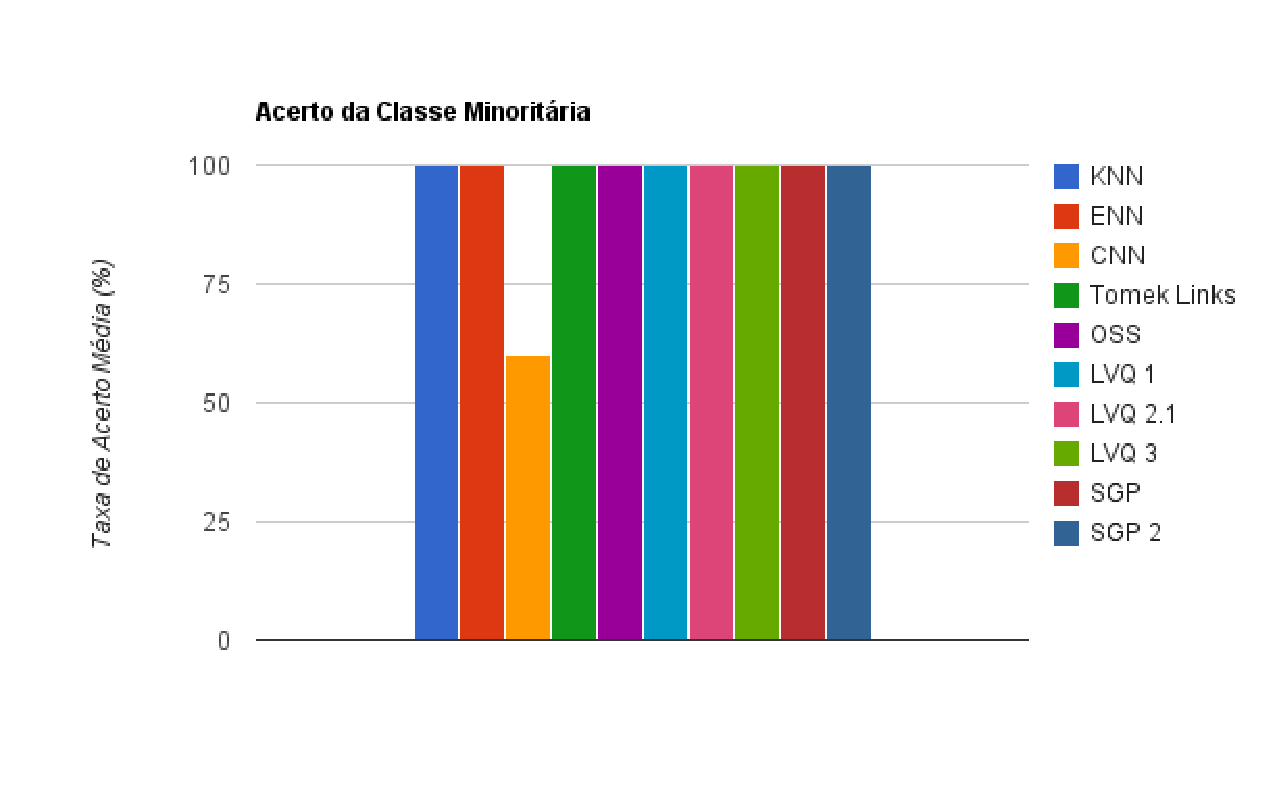
\includegraphics[scale=0.80]{imagens/graficos/grafico1_iris.eps}
\caption{Taxa de acerto da classe minorit�ria por t�cnica na base Iris}
\label{fig:iris1}
\end{figure}

O OSS, t�cnica utilizada para bases desbalanceadas, obteve uma taxa de acerto total de 84.18\% em m�dia, uma taxa de acerto baixa em rela��o as outras t�cnicas. A redu��o tamb�m n�o foi t�o alta, a quantidade de prot�tipos resultantes foi em m�dia 34.18\% da baso original. Por�m, como o \textit{One-Sided Selection} d� prioridade a classe minorit�ria, pode-se observar que a taxa de acerto desta classe foi de 100\%, o que torna esta uma t�cnica eficiente quando o caso de interesse � a classe minorit�ria.

O LVQ 1, 2.1 e 3 n�o tiveram diferen�a entre si, provavelmente isso se deve ao fato de as classes estarem bem separadas. Uma caracter�stica interessante � que as vers�es do \textit{Learning-Vector Quantization} obtiveram quase 99.31\% de acerto total, sendo a taxa de acerto para classe minorit�ria de 100\%. Isso comprova o que foi dito no cap�tulo anterior, o LVQ � eficiente para bases desbalanceadas, principalmente quando as classes est�o bem separadas. O poder de redu��o desta classe tamb�m tem um bom desempenho, visto que � poss�vel escolher a quantidade de prot�tipos finais, assim como corrigir o desbalanceamento.

Como a base Iris0 possui baixo n�vel de desbalanceamento, as duas vers�es do \textit{Self-Generating Prototypes} obtiveram um excelente desempenho. A taxa de acerto geral para ambas foi de 98.64\%, uma excelente taxa, considerando que a quantidade de prot�tipos resultante foi de 1.70\% do conjunto de treinamento original. Esta t�cnica possui um alto poder de redu��o, e nesta base, a taxa de acerto da classe minorit�ria foi de 100\%.

N�o houve diferen�a entre o SGP1 e SGP2, pois a separa��o entre as classes tornou os passos de $Merge$ e $Pruning$ desnecess�rios.

\begin{figure}[H]
\center
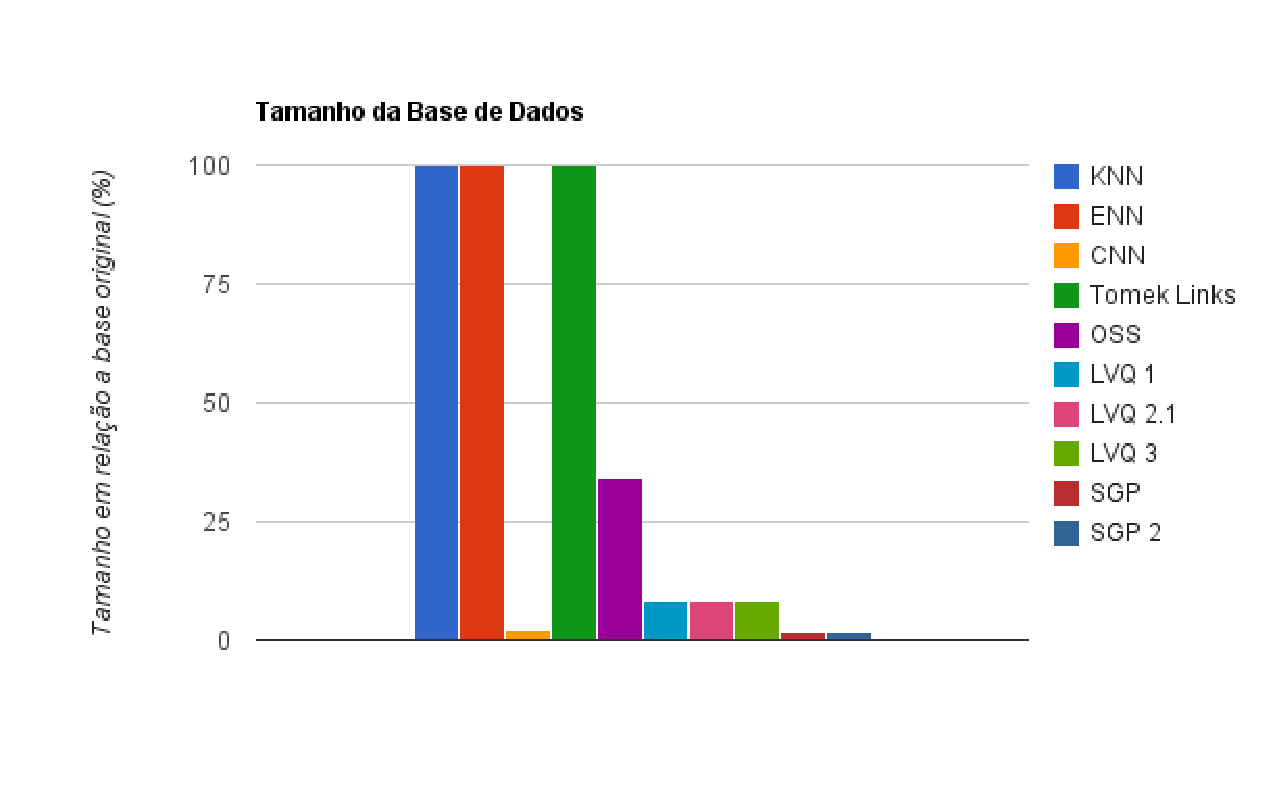
\includegraphics[scale=0.80]{imagens/graficos/grafico2_iris.eps}
\caption{Tamanho a base de dados ap�s sele��o de prot�tipos na base Iris}
\label{fig:iris2}
\end{figure}

Nesta base, com regi�es de baixa sobreposi��o de classes, o ENN e o Tomek Links foram in�teis, pois n�o apresentaram redu��o de dados. J� o CNN se mostrou altamente ineficiente, pois reduziu tanto a classe minorit�ria (para uma inst�ncias) que tornou a taxa de acerto desta classe nula, pois foi utilizado K=3.

Com este experimento, conclui-se tamb�m que, em bases com baixo n�vel de desbalanceamento e boa separa��o entre as classes, as vers�es do \textit{Self-Generating Prototypes} s�o eficientes e possuem um alto poder de redu��o. Por�m, t�cnicas como o \textit{Learning-Vector Quantization} podem ser ainda mais eficientes, principalmente com a escolha adequada de par�metros, al�m de n�o correr risco de elimina��o da classe minorit�ria.

Outra t�cnica apropriada para este tipo de base foi o \textit{One-Sided Selection}. Por priorizar a classe minorit�ria, o OSS garante uma boa taxa de acerto para esta classe. Por�m, comparando esta t�cnica com o SGP e LVQ, percebe-se que ela tem um baixo n�vel de redu��o, sendo recomendado a aplica��o de outra t�cnica ap�s o OSS.



\section{Glass 5}

A base Glass5 � uma base com alto desbalanceamento. Esta base cont�m 214 inst�ncias, cada uma contendo nove atributos. Apenas 4.20\% das inst�ncias s�o da classe minorit�ria, \textit{tableware}, e 95.80\% da classe marjorit�ria, \textit{reminder}.


\begin{table}[H]\tiny
\begin{center}
\begin{tabular}{|@{}l@{}|@{}l@{}|@{}l@{}|@{}l@{}|@{}l@{}|@{}l@{}|@{}l@{}|@{}l@{}|@{}l@{}|@{}l@{}|@{}l@{}|}
\hline
T�cnica		    &KNN&ENN&CNN&Tomek Links&OSS&LVQ 1&LVQ 2.1&LVQ 3&SGP&SGP 2 \\
\hline %----- linha horizontal
Acerto Total		    & 96.28 $\pm$ 3.53 \%& 95.81 $\pm$ 2.55 \%& 95.80 $\pm$ 1.02 \%& 96.28 $\pm$ 3.53 \%& 85.53 $\pm$ 15.62 \%& 80.35 $\pm$ 4.65 \%& 81.28 $\pm$ 5.81 \%& 81.30 $\pm$ 5.98 \%& 95.80 $\pm$ 1.93 \%& 95.80 $\pm$ 1.93 \% \\
\hline
Acerto Marjorit�ria		   & 98.05 $\pm$ 3.18 \%& 99.02 $\pm$ 2.18 \%& 100.00 $\pm$ 0.00 \%& 98.05 $\pm$ 3.18 \%& 86.83 $\pm$ 16.60 \%& 80.98 $\pm$ 5.56 \%& 81.95 $\pm$ 6.36 \%& 81.46 $\pm$ 6.59 \%& 99.51 $\pm$ 1.09 \%& 99.51 $\pm$ 1.09 \% \\
	\hline
Acerto Minorit�ria		    & 60.00 $\pm$ 41.83 \%& 30.00 $\pm$ 44.72 \%& 0.00 $\pm$ 0.00 \%& 60.00 $\pm$ 41.83 \%& 60.00 $\pm$ 41.83 \%& 60.00 $\pm$ 54.77 \%& 60.00 $\pm$ 54.77 \%& 70.00 $\pm$ 44.72 \%& 10.00 $\pm$ 22.36 \%& 10.00 $\pm$ 22.36 \% \\
\hline
Tamanho Resultante		     & 100.00 $\pm$ 0.00 \%& 95.78 $\pm$ 1.13 \%& 7.86 $\pm$ 1.24 \%& 99.30 $\pm$ 0.64 \%& 10.67 $\pm$ 0.88 \%& 5.86 $\pm$ 0.03 \%& 5.86 $\pm$ 0.03 \%& 5.86 $\pm$ 0.03 \%& 3.17 $\pm$ 1.59 \%& 1.64 $\pm$ 1.46 \% \\
\hline
\end{tabular}%--- fechaoento do aobiente tabular
\end{center}   %fio da centraliza��o da tabela
\caption{Tabela do Glass 5}
\label{tab:glass}
\end{table}

\begin{figure}[H]
\center
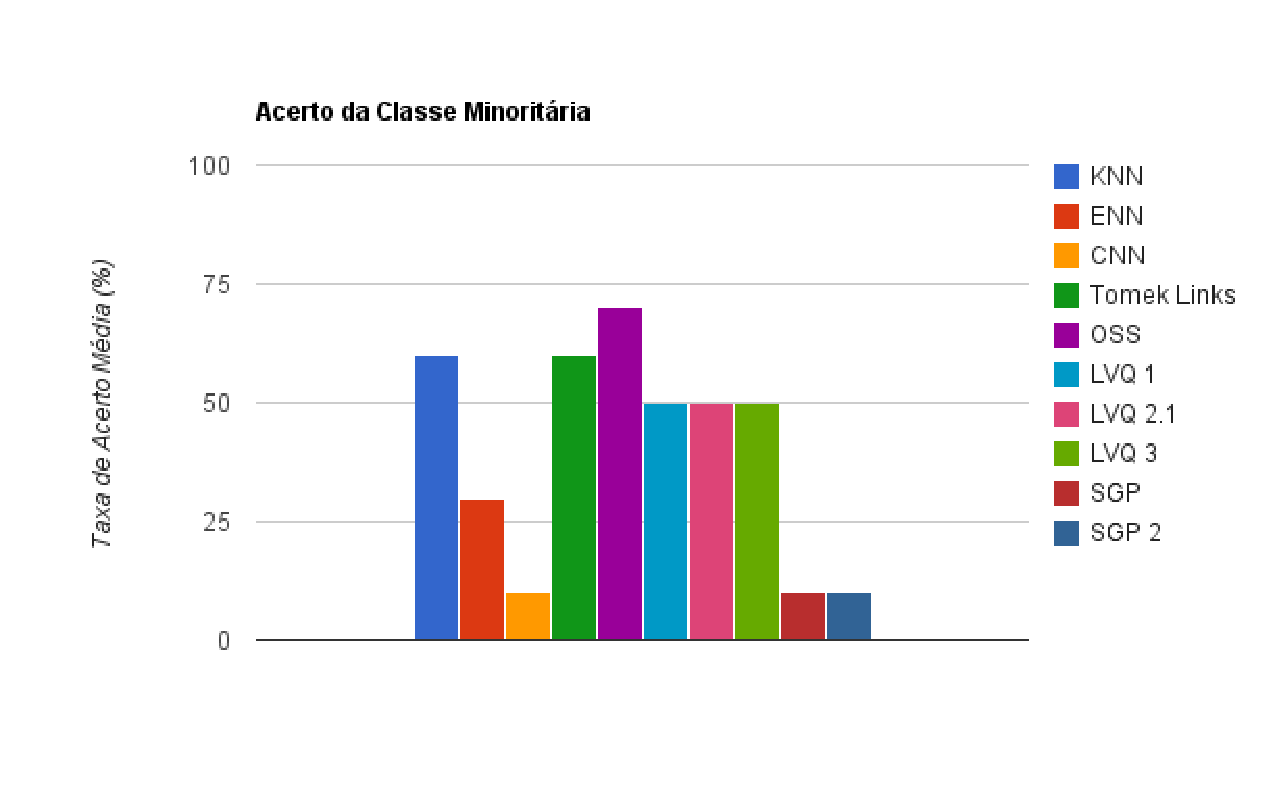
\includegraphics[scale=0.80]{imagens/graficos/grafico1_glass.eps}
\caption{Taxa de acerto da classe minorit�ria por t�cnica na base Glass}
\label{fig:glass1}
\end{figure}


\begin{figure}[H]
\center
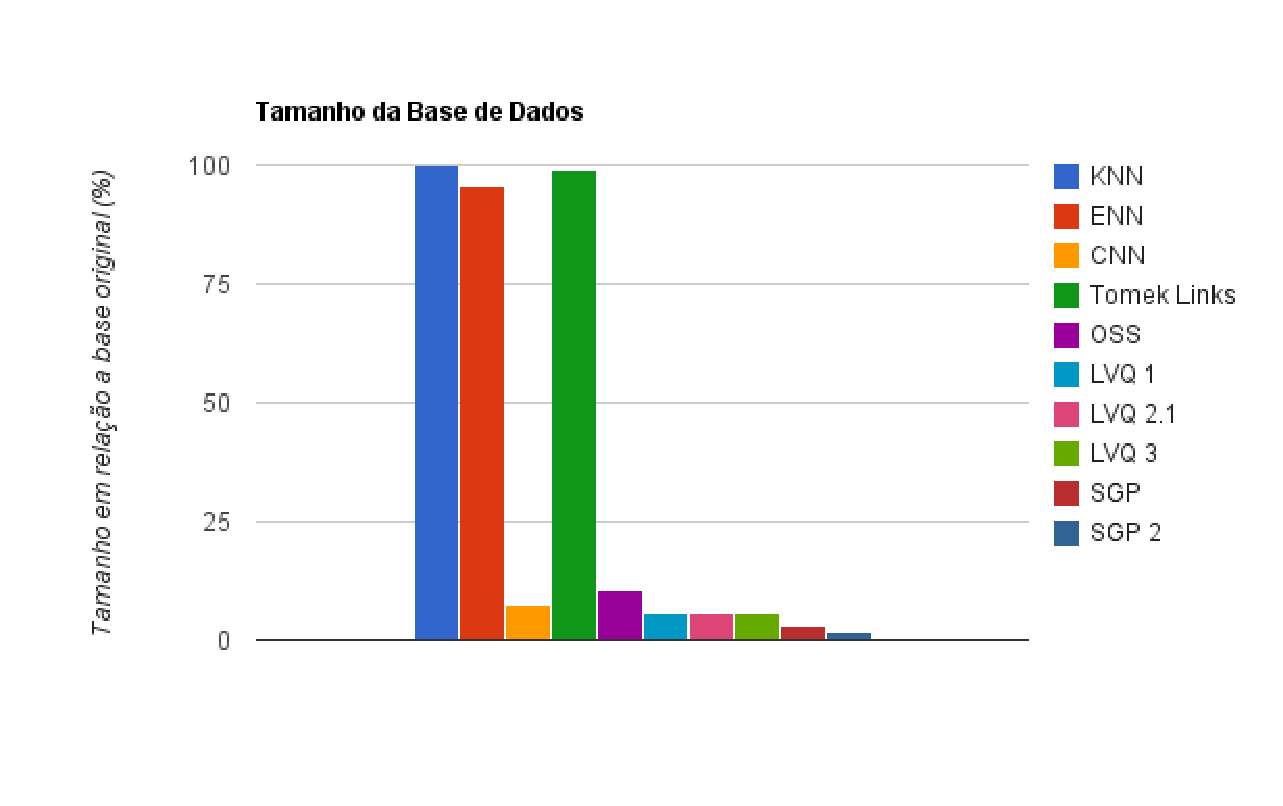
\includegraphics[scale=0.80]{imagens/graficos/grafico2_glass.eps}
\caption{Tamanho a base de dados ap�s sele��o de prot�tipos na base Glass}
\label{fig:glass2}
\end{figure}


Observando a tabela \ref{tab:glass}, percebe-se que, neste exemplo, al�m de a base ser mais desbalanceada, existe uma maior sobreposi��o de classes que o exemplo anterior. Em geral, as t�cnicas obtiveram uma boa taxa de acerto geral, mas a taxa de acerto da classe minorit�ria variou muito de acordo com a t�cnica.

Como a base Glass 5 apresenta sobreposi��o de classes, o ENN gerou uma pequena redu��o de inst�ncias, reduzindo para 95.78\% em m�dia. Por�m, a taxa de acerto da classe minorit�ria foi muito pequena em rela��o a marjorit�ria. o ENN obteve uma taxa m�dia de 30\% de acerto e desvio padr�o foi de 44.72\% na classe minorit�ria, assim, conforme comprovado nas bases artificiais, quando existe uma maior sobreposi��o, a classe minorit�ria � muito reduzida, compromentendo grandemente o desempenho do classificador para esta classe.

J� o CNN conseguiu reduzir consideravelmente o n�mero de inst�ncias, mas sua taxa de acerto para bases desbalanceadas foi praticamente nula. Isso confirma o que foi visto na base Iris 0, o CNN n�o � uma t�cnica eficiente para bases desbalanceadas, principalmente com alto n�vel de desbalanceamento. Com a modifica��o do CNN usada pelo OSS, a taxa de acerto seria melhorada, mas a t�cnica tradicional mais uma vez n�o se mostrou apropriada para o caso de estudo.

O Tomek Links conseguiu uma boa taxa de acerto m�dia, 96.28\%, se comparado com as t�cnicas anteriores. A taxa de acerto da classe minorit�ria foi de 60\%. Se comparado com o KNN, observa-se que o Tomek Links foi eficiente para classificar bases desbalanceadas, mas isso aconteceu porque o Tomek Links praticamente n�o alterou a base de dados, sendo a quantidade de prot�tipos selecionados 99.30\% do conjunto de treinamento original. Com isso, conclui-se que o Tomek Links � eficiente na remo��o de inst�ncias na regi�o de indecis�o, por�m, nem sempre a regi�o de indecis�o � significativa em rela��o a original, assim, recomenda-se o uso de sua vers�o adaptada como pr�-processamento.

O OSS, obteve uma taxa de acerto total inferior as t�cnicas citadas anteriormente, sendo 85.53\% em m�dia. Todavia, observa-se que a taxa de acerto da base minorit�ria foi de 60\%, a mesma taxa do KNN e, diferentemente do Tomek Links, a quantidade de prot�tipos selecionados pelo OSS foi em m�dia apenas 10.67\% do conjunto de treinamento original. Isso mostra que, mesmo com um n�vel de desbalanceamento maior, \textit{One-Sided Selection} tem um alto poder de redu��o e prioriza a classe minorit�ria.

As vers�es do LVQ tiveram desempenho parecido, por�m, o LVQ 3 se mostrou mais eficiente para a classe minorit�ria. Observando os experimentos do cap�tulo anterior, percebe-se que, neste experimento, o espalhamento controlado dos prot�tipos resultou em um aumento percentual da taxa de acerto da classe minorit�ria de 10\% em rela��o as outras vers�es do LVQ.

Comparando o LVQ 3 com as t�cnicas anteriores, percebe-se que ele teve um alto n�vel de redu��o da base, apenas 5.86\% de inst�ncias foram necess�rias para ter a mesma taxa de acerto da classe minorit�ria que o pr�prio KNN.

O \textit{Learning Vector Quantization} � uma t�cnica eficiente, e percebe-se que, ao diminuir o desbalanceamento de classes, esta t�cnica beneficia casos onde a classe minorit�ria � o caso de interesse e, ainda assim, n�o compromete, consideravelmente, a taxa de acerto da classe marjorit�ria.

O \textit{Self-Generating Prototypes 1} foi altamente ineficiente em classificar a classe minorit�ria. A tabela \ref{tab:glass} mostra que o SGP 1 reduziu a base de dados para 3.17\% do conjunto de treinamento original, mas o custo disso foi uma taxa de acerto m�dia de apenas 10\% para classe minorit�ria. No caso da Iris 0, como existia um baixo n�vel de desbalanceamento o SGP foi eficiente, por�m, com uma base mais desbalanceada, esta t�cnica removeu a maioria das inst�ncias da classe minorit�ria, tornando os prot�tipos resultantes invi�veis para qualquer classificador.

A segunda vers�o do SGP teve o mesmo comportamento que o SGP 1, por�m, o reduziu a base para 1.64\%. Esta redu��o seria interessante, caso o SGP 1 tivesse tido um bom desempenho, mas, como n�o foi o caso, o SGP 2 tamb�m se mostrou invi�vel.


Assim, conclui-se que, em bases com alto n�vel de desbalanceamento e com sobreposi��o de classes, as vers�es do SGP s�o invi�veis, principalmente quando o caso de interesse � a classe minorit�ria. J� o LVQ, mais uma vez se mostrou eficiente para identifica��o da classe minorit�ria, mostrando que a elimina��o do desbalanceamento � uma estrat�gia interessante para este caso.

Da mesma forma que o experimento anterior, o OSS teve um bom desempenho para classificar inst�ncias da classe minorit�ria, sendo recomendado mesmo com alto n�vel de desbalanceamento.


\section{Yeast 6}

A base Yesat 6 � a base de mais alto n�vel de desbalanceamento estudada neste trabalho. Esta base cont�m 1484 inst�ncias, cada uma contendo 8 atributos. Apenas 2.49\% das inst�ncias s�o da classe minorit�ria, \textit{exc}, e 97.51\% da classe marjorit�ria, \textit{reminder}.

\begin{table}[H]\tiny
\begin{center}
\begin{tabular}{|@{}l@{}|@{}l@{}|@{}l@{}|@{}l@{}|@{}l@{}|@{}l@{}|@{}l@{}|@{}l@{}|@{}l@{}|@{}l@{}|@{}l@{}|}
\hline
T�cnica		    &KNN&ENN&CNN&Tomek Links&OSS&LVQ 1&LVQ 2.1&LVQ 3&SGP&SGP 2 \\
\hline %----- linha horizontal
Acerto Total		    & 97.63 $\pm$ 0.96 \%& 98.04 $\pm$ 0.81 \%& 97.29 $\pm$ 1.35 \%& 97.90 $\pm$ 0.94 \%& 96.41 $\pm$ 1.28 \%& 86.86 $\pm$ 2.15 \%& 87.07 $\pm$ 2.18 \%& 87.13 $\pm$ 2.45 \%& 97.77 $\pm$ 0.91 \%& 97.36 $\pm$ 0.80 \% \\
\hline
Acerto Marjorit�ria		   & 98.96 $\pm$ 0.49 \%& 99.44 $\pm$ 0.53 \%& 98.41 $\pm$ 1.31 \%& 99.10 $\pm$ 0.53 \%& 97.16 $\pm$ 0.93 \%& 86.82 $\pm$ 2.21 \%& 87.03 $\pm$ 2.25 \%& 87.10 $\pm$ 2.55 \%& 98.96 $\pm$ 0.65 \%& 98.54 $\pm$ 0.45 \% \\
\hline
Acerto Minorit�ria		    & 42.86 $\pm$ 22.59 \%& 40.00 $\pm$ 23.47 \%& 51.43 $\pm$ 12.78 \%& 48.57 $\pm$ 23.90 \%& 65.71 $\pm$ 16.29 \%& 88.57 $\pm$ 11.95 \%& 88.57 $\pm$ 11.95 \%& 88.57 $\pm$ 11.95 \%& 48.57 $\pm$ 25.95 \%& 48.57 $\pm$ 32.89 \% \\
\hline
Tamanho Resultante		     & 100.00 $\pm$ 0.00 \%& 97.94 $\pm$ 0.30 \%& 6.44 $\pm$ 0.74 \%& 98.80 $\pm$ 0.24 \%& 8.46 $\pm$ 1.01 \%& 0.86 $\pm$ 0.00 \%& 0.86 $\pm$ 0.00 \%& 0.86 $\pm$ 0.00 \%& 9.24 $\pm$ 1.66 \%& 4.66 $\pm$ 0.80 \% \\
\hline
\end{tabular}%--- fechaoento do aobiente tabular
\end{center}   %fio da centraliza��o da tabela
\caption{Tabela do Yeast 6}
\label{tab:yeast}
\end{table}

\begin{figure}[H]
\center
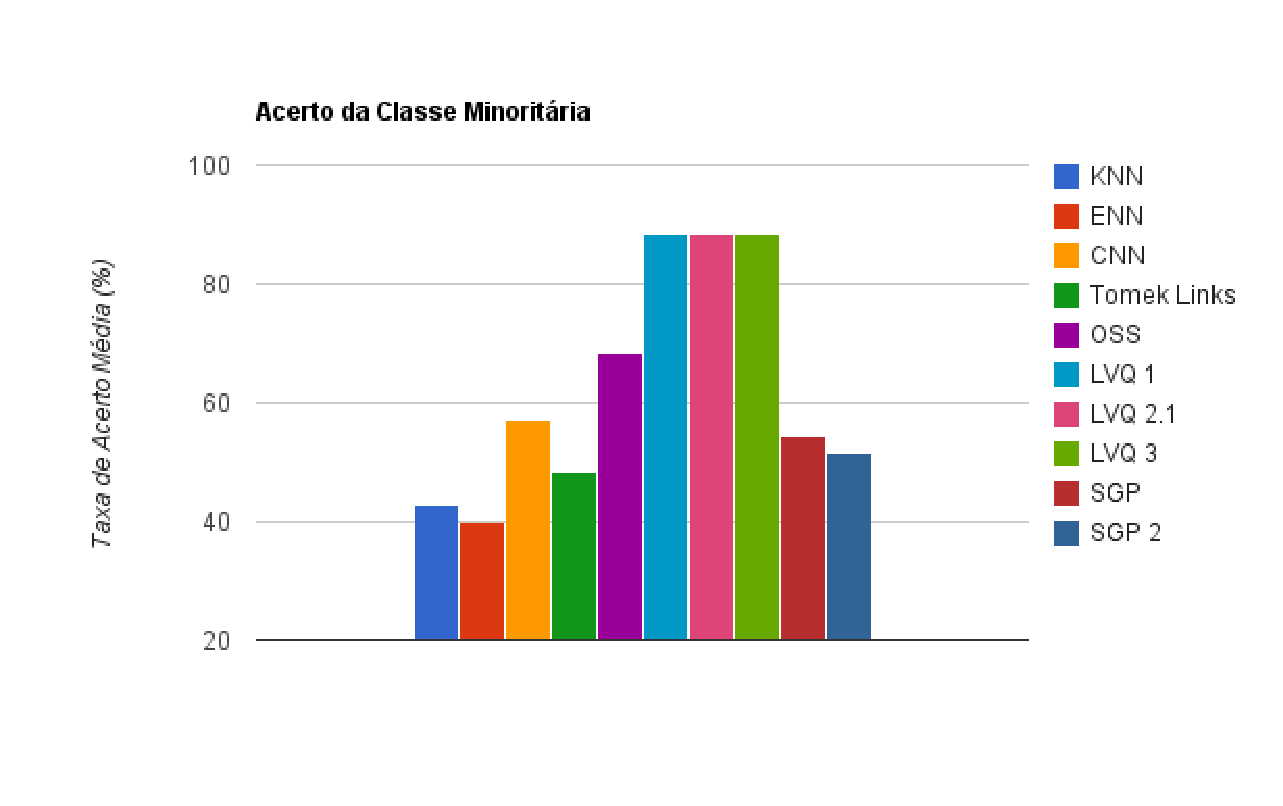
\includegraphics[scale=0.80]{imagens/graficos/grafico1_yeast.eps}
\caption{Taxa de acerto da classe minorit�ria por t�cnica na base Yeast}
\label{fig:yeast1}
\end{figure}

A base Yeast 6 � de mais alto n�vel de desbalanceamento e ser� o referencial para casos extremos neste trabalho.

Observando a tabela \ref{tab:yeast} percebe-se que o KNN teve uma taxa de acerto alta, por�m, a taxa de acerto da classe minorit�ria foi em m�dia apenas 42.86\%.

\begin{figure}[H]
\center
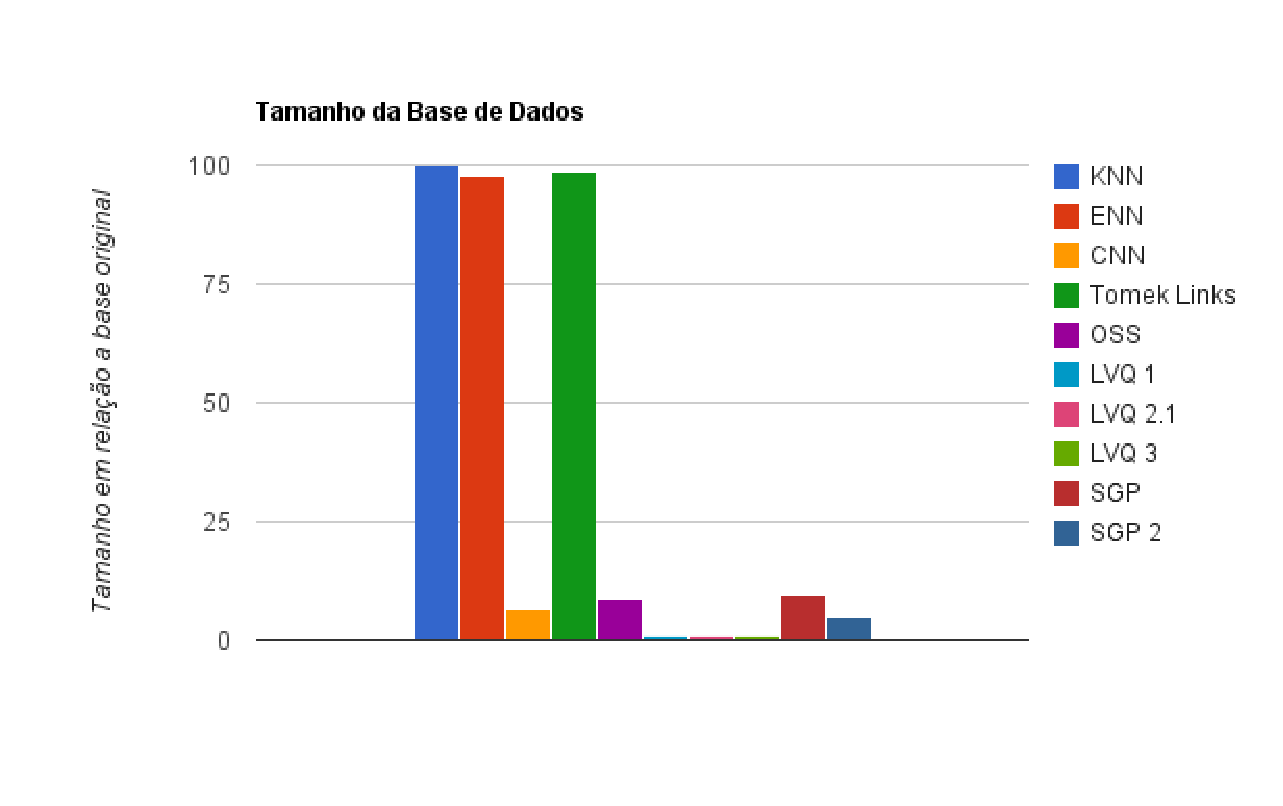
\includegraphics[scale=0.80]{imagens/graficos/grafico2_yeast.eps}
\caption{Tamanho a base de dados ap�s sele��o de prot�tipos na base Yeast}
\label{fig:yeast2}
\end{figure}

O ENN reduziu a base de dados para 97.94\% e aumentou a taxa de acerto geral para 98.04\%, mas o custo disso foi a redu��o da taxa de acerto da classe minorit�ria em 2.86\% em m�dia. 

J� o CNN, por manter inst�ncias da regi�o de fronteira e, neste caso, praticamente todas as inst�ncias da classe minorit�ria, foi eficiente. Os prot�tipos selecionados por esta t�cnica foram apenas 6.44\% do conjunto de treinamento, ou seja, diminuiu consideravelmente o custo e o tempo de processamento. Al�m desta redu��o, o CNN teve um aumento de 8.57\% na taxa de acerto da classe minorit�ria em rela��o ao KNN.

O Tomek Links, apesar de tamb�m remover inst�ncias da classe minorit�ria, apresentou uma melhora em rela��o ao KNN. Esta t�cnica apresentou um ganho de 5.71\% na taxa de acerto da classe minorit�ria em m�dia. O desvio padr�o, por�m, mostra que houve casos onde a taxa de acerto foi inferior a 30\%, ou seja, o Tomek Links deve ser utilizado apenas quando a quantidade de inst�ncias removidas n�o ser� significativa para a classifica��o.

O OSS se mostrou a t�cnica seletiva mais eficiente. Por utilizar o CNN modificado o n�vel de desbalanceamento foi reduzido e o Tomek Links modificado deixou a classe minorit�ria bem definida, assim, a taxa de acerto da classe minorit�ria foi de 65.71\%, o que representa um aumento de 22.85\% em rela��o ao KNN. Mais uma vez, o OSS se mostrou eficiente independente do n�vel de desbalanceamento e sobreposi��o de classes.

Entre as vers�es do LVQ n�o houve diferen�a relevante. Mesmo neste caso extremo o LVQ teve uma taxa de acerto m�dia de 88.57\%, sendo superior ao OSS. Isso mostra que, como o LVQ elimina o desbalanceamento, a classe minorit�ria � extremamente beneficiada. Outra vantagem do LVQ � a redu��o de inst�ncias, nesta base, a quantidade de prot�tipos foi apenas 0.86\% do conjunto de treinamento.

O SGP 1 teve um bom desempenho se comparado com o KNN. A taxa de acerto da classe minorit�ria foi de 48.57\%, isso �, um aumento de 5.71\% em rela��o ao KNN. Al�m disso, os prot�tipos criados por esta t�cnica foram apenas 9.24\% do conjunto original. Por�m, se comparado com o LVQ, percebe-se que o SGP teve uma redu��o baixa e n�o priorizou a classe minorit�ria. Na base Yast 6, o SGP 2 teve o mesmo desempenho que o SGP, por�m, reduziu a base para 4.66\% do conjunto de treinamento original.

Apesar de terem um bom desempenho m�dio nesta base, as duas vers�es do SGP n�o s�o recomendadas em bases desbalanceadas. Em alguns folds, o SGP 2 teve uma taxa de acerto da classe minorit�ria inferior a 25\%, isso aconteceu porque neste fold, as inst�ncias n�o ficaram agrupadas, e foram totalmente eliminadas na aplica��o do fator de generaliza��o.


Com este experimento, conclui-se que, em base altamente desbalanceadas o OSS � muito eficiente e recomendado, assim como o LVQ, isso acontece pelos motivos j� citados em sess�es anteriores.

O ENN se mostrou altamente ineficiente por remover grande quantidade de inst�ncias da classe minorit�ria, o mesmo aconteceu com o SGP 1 e 2, e, em alguns casos com o Tomek Links.

Uma t�cnica que se comportou de forma diferente dos experimentos anteriores foi o CNN que se mostrou eficiente. Neste caso, pode-se dizer que as inst�ncias da classe minorit�ria est�o distribu�das e a maioria das inst�ncias desta classe foram selecionadas. Ou seja, para o uso do CNN, � importante que a classe minorit�ria esteja bem distribu�da para que mais inst�ncias desta classe sejam selecionadas.


% !TEX encoding = ISO-8859-1
\chapter{Conclus�o}
% \label{ch:introducao}

\section{Considera��es Finais}

	Com os experimentos realizados conclui-se que t�cnicas como o \textit{Edited Nearest Neighbor} e \textit{Tomek Links} em suas vers�es originais s�o eficientes para remo��o de ru�dos, por�m, para bases desbalanceadas ela pode remover todas as inst�ncias da classe minorit�ria, tornando a base invi�vel para qualquer classificador. Para uso destas t�cnicas, recomenda-se uma adapta��o para n�o remover inst�ncias da classe minorit�ria.

	O \textit{Condensed-Nearest Neighbor} pode ser eficiente, dependendo da sobreposi��o de classes. Em casos onde as classes est�o bem separadas, o uso do CNN s� deve ser feito caso o classificador considere apenas a inst�ncia mais pr�xima. Caso o classificador seja um 3-NN, esta t�cnica pode deixar apenas um prot�tipo da classe minorit�ria, tornando-a invi�vel, mesmo para pr�-processamento. Para o CNN uma boa op��o � utilizar sua vers�o adaptada.

	A t�cnica que se mostrou muito eficiente foi o \textit{One-Sided Selection}. Esta t�cnica foi eficiente em identificar a classe minorit�ria em todos os experimentos, independente do n�vel de sobreposi��o e desbalanceamento. Por�m, esta t�cnica possui um baixo poder de redu��o de inst�ncias, sendo recomendado utilizar o OSS como t�cnica de pr�-sele��o de prot�tipos.

	Assim como o OSS, as vers�es do \textit{Learning Vector Quantization}, ao reduzir o n�vel de desbalanceamento favorece a classe minorit�ria. Independente do n�vel de sobreposi��o, esta t�cnica se mostrou eficiente. Um defeito desta t�cnica � que ela possui muitos par�metros, ent�o, a escolha dos valores adequados pode tornar o processo de treinamento lento.

	As duas vers�es do \textit{Self-Generating Prototypes} s�o muito eficientes para bases com baixo n�vel de desbalanceamento e sobreposi��o. Mas ambas as vers�es possuem um p�ssimo desempenho em classificar inst�ncias da classe minorit�ria quando existe um alto desbalanceamento e sobreposi��o de classes. Recomenda-se n�o utilizar esta t�cnicas com fator de generaliza��o para evitar a elimina��o da classe minorit�ria em bases desbalanceadas.

	Ap�s analisar todas as t�cnicas, percebe-se que aquelas que tratam a classe minorit�ria de forma especial possuem um melhor desempenho em identificar esta classe do que t�cnicas que tratam todas as classes igualmente. Ent�o, recomenda-se o uso de t�cnicas que diminuam o desbalanceamento antes de aplicar t�cnicas tradicionais de sele��o de prot�tipos, para que haja efici�ncia em identificar a classe minorit�ria.

\section{Trabalhos Futuros}

	Percebendo que t�cnicas adaptadas para classes desbalanceadas com o \textit{One-Sided Selection} possuem um bom desempenho, � de se esperar que o \textit{Self-Generating Prototypes} que trate as classes marjorit�ria e minirit�ria de formas distintas seja tamb�m eficiente.

	O SGP 1 e 2 possuem um alto poder de redu��o de inst�ncias e se mostraram muito eficiente em bases com baixo n�vel de desbalanceamento. Para trabalhos futuros, uma adapta��o no SGP pode gerar uma t�cnica que mantenha as caracter�sticas de representa��o de classes, mas que promova uma redu��o no desbalanceamento, pode ser muito eficiente.

	Uma adapta��o percept�vel atrav�s dos experimentos deste trabalho � utilizar fatores de generaliza��o diferentes para a classe marjorit�ria e para minorit�ria. Isso pode ser feito utilizando o maior grupo de uma classe $C$ para eliminar um grupo da classe $C$, e n�o o maior grupo da base. Para o SGP 2, as fases de $Merge$ e $Pruning$ podem ser feitas apenas com grupos da classe marjorit�ria.

	Com estas adapta��es sugeridas, o SGP ter� as mesmas caracter�sticas de redu��o de inst�ncias e representatividade das classes, mas favorecer� a identifica��o da classe minorit�ria, assim como o OSS.








%% Parte p�s-textual
\backmatter

\appendix
% !TEX encoding = ISO-8859-1
\chapter{Figuras das Bases Artificiais}
\label{ch:appendixa}

\section{Figuras com 10\% da classe minorit�ria}
\begin{figure}[H]
\center
	\mbox{%
		\subfigure[N�vel I de sobreposi��o]{\label{fig:orig100}%
			\includegraphics[scale=0.30]{imagens/outputs/ORIG_10_0.eps}} 
		\subfigure[N�vel II de sobreposi��o]{\label{fig:orig101}%
			\includegraphics[scale=0.30]{imagens/outputs/ORIG_10_1.eps}}
	}
	\mbox{%
		\subfigure[N�vel III de sobreposi��o]{\label{fig:orig105}%
			\includegraphics[scale=0.30]{imagens/outputs/ORIG_10_5.eps}}
		\subfigure[N�vel IV de sobreposi��o]{\label{fig:orig1010}%
			\includegraphics[scale=0.30]{imagens/outputs/ORIG_10_10.eps}}
    }
	\mbox{%
		\subfigure[N�vel V de sobreposi��o]{\label{fig:orig1015}%
			\includegraphics[scale=0.30]{imagens/outputs/ORIG_10_15.eps}} 
    }
  \caption{Bases artificiais com 10\% da classe minorit�ria}
  \label{fig:orig:10}
\end{figure}

\section{Figuras com 5\% da classe minorit�ria}
\begin{figure}[H]
\center
	\mbox{%
		\subfigure[N�vel I de sobreposi��o]{\label{fig:orig50}%
			\includegraphics[scale=0.30]{imagens/outputs/ORIG_10_0.eps}} 
		\subfigure[N�vel II de sobreposi��o]{\label{fig:orig51}%
			\includegraphics[scale=0.30]{imagens/outputs/ORIG_10_1.eps}}
	}
	\mbox{%
		\subfigure[N�vel III de sobreposi��o]{\label{fig:orig55}%
			\includegraphics[scale=0.30]{imagens/outputs/ORIG_10_5.eps}}
		\subfigure[N�vel IV de sobreposi��o]{\label{fig:orig510}%
			\includegraphics[scale=0.30]{imagens/outputs/ORIG_10_10.eps}}
    }
	\mbox{%
		\subfigure[N�vel V de sobreposi��o]{\label{fig:orig515}%
			\includegraphics[scale=0.30]{imagens/outputs/ORIG_10_15.eps}} 
    }
  \caption{Bases artificiais com 5\% da classe minorit�ria}
  \label{fig:orig5}
\end{figure}






% Bibliografia
\nocite{*}
\bibliographystyle{alpha}
\bibliography{bibliografia/bibliografia}

% \colophon % UFPEThesis reference

\end{document}
